\cotefile{15}
\scanpage{195}
2°) $X_{\deleted{\unsure{\mathrm{réd}}}}$ domine $\operatorname{Spec}\mathbf Z$, i.e. $X$ contient des pts de car. résiduelle nulle.

Alors \deleted{\unsure{en plus} \inserted{\unsure{dispose}} \deleted{\unsure{de}} \unsure{de ceci} (et éventuellement \unsure{cristalline} \unsure{le cas d'inégales car.}) on a, pour \unsure{tt pt}}

\deleted{\unsure{ét. (crist.)}}

(i) $\xi_\ell\in\unsure{\mathbf T}(\mathbf Z_\ell)$ \uline{\unsure{tt}} $\ell\in\mathbf P$, $\xi_\ell$ provenant d'un \unsure{élém.} de $T_{\unsure{\alpha}}(\widetilde{\mathbf Z}_{\unsure{\ell\mathbf Z}})$.

$\xi_\ell$ dépend du choix d'un pt géom. quelconque de $X$, et est indép. de ce choix modulo opération du $\pi_1$, notation $\xi_{\bar x,\ell}:=\xi_{X,\ell}$.

(ii) Si $X$ a des points $x$ de car. $p>0$, alors on dispose également des $\xi_{x,p}$, $\xi_{x,p}^{0}$.

\unsure{Connexions} : \unsure{relation}, \deleted{\unsure{de la}} si $y$ est un pt de car. $p>0$ et \deleted{\unsure{$x$}} un pt de car. $0$, entre $\xi_{y,p}$ et $\xi_{x,p}\otimes_{\mathbf Z_p}W(k)$ [$y$ pt \unsure{à val.} sur un corps parfait $k$].

\uline{Ils ne sont en général pas semi-simples}, sans doute. \deleted{\unsure{Ils}} \unsure{Si} \deleted{\unsure{sont semi-simples}} leurs \unsure{poids}, ils sont cependant semi-simples \unsure{par le gr.}, \deleted{\unsure{et les $\xi_p$ doivent}} \deleted{\illegible{6}}.
\margin{\uuline{\deleted{\unsure{Vérifier}}}$\longrightarrow$}

(iii) Si $x$ est un pt \unsure{à val. ds.} un corps \inserted{$k$} de \uline{car. $0$}, on a $\xi_{x,\infty}\in T_{\unsure{\alpha}}(k)$ par Hodge-de Rham. Il n'y a pas lieu de \inserted{Avec ses \textcircled{\uuline{2}} filtrations \deleted{\unsure{algébriques}} !}

\margin{L'une est celle \unsure{qui} donne comme gr. associé les $\unsure{H^i}(x,\unsure{\Omega^j})$, l'autre (arithmétique) \deleted{\unsure{par}} \unsure{provient de} la filtration canonique des motifs. (Elle est \uline{triviale} pour les motifs simples) La première filtration est \unsure{originelle} au foncteur Hodge-De Rham, bien faire attention qu'elle ne provient pas d'une filtration des motifs, c'est une filtration du \uline{\unsure{foncteur}} !}
\margin{194}
\scanpage{196}
\margin{195}
ALGÈBRES de LIE SEMI-SIMPLES (7) \hfill Tribu n° 59

mettre l'exer. 1, (p. 36), en c) de la prop. 11, et l'exer. 2 dans le texte.

Ajouter un utile rabiot sur les algèbres de la forme, (commutative), $\times\underline{\mathrm{sl}}_2$, à savoir les généralisations des prop. 5 et 6.

\S 3 -- \uuline{Le système de racines...}

\uline{n° 1} -- Définir ``déploiement'', (i.e. couple $(\underline g,\underline h)$), ``déployable''. Dire que $(*)$ de la déf. 1 signifie que $\operatorname{ad}(x)$ est diagonalisable, (on sait qu'il est semi-simple). Ajouter ``semi-simple'' à la l.2 bas, (p. 37).

Remplacer ``canonique'' par ``diagonale'', et ``abélienne'' par ``commutative'', ousqui faut.

\uline{n° 2} -- Il s'agit du sous-espace ``primaire'' à la p. 38, l.4. A la l.5 dire : ``comme $\operatorname{ad}(\underline h)$ est semi-simple, $\underline g^\alpha$ est l'ensemble...'', et ne pas répéter ça à la l.16. Dans l'énoncé du th. 2 dire que $\underline h^\alpha$ est un sous-espace de dim. 1 de $\underline h$. Y expliciter l'isom. $\varphi_\alpha$ dans (iii). Ajouter ``et si'' dans le (iv).

\uline{n° 3} -- Après le premier alinéa de la p. 41, démontrer le th. 3, c), (cf. p. 44), ce qui règle son compte au th. 3. Plus bas utiliser l'isom. $\varphi_\alpha$. Commencer la p. 42 par ``Soit...''. A la l.3, (p. 42), qualifier $W(2)$ de ``module simple''. Ce qui est entre parenthèses en-dessous est maintenant fait au \S 2. Dire, (p. 42, l.12), que $R$ est un système de racines `` de $\underline h$ ''.

Le haut de la p. 44 remonte p. 41.

\uline{n° 4} -- Titre : terminologie et inventaire.

\uline{n° 5} -- A la l.2 bas de la p. 45 dire : ``Dans tout couple $(\alpha,-\alpha)$ de racines opposées, choisissons arbitrairement une racine $\alpha$ ; pour chaque racine $\alpha$ ainsi choisie, choisissons... $X_\alpha$...''.
\scanpage{197}
penser que pour les \unsure{pts différents} à val. dans $\unsure{k_0}\subset k$, les deux foncteurs obtenus, soient \unsure{isom.} (pas plus que dans le cas (ii)). Il n'y a plus en général d'opération de $\pi_1(X)$ sur $\xi_{x,\infty}$, mais encore comme dans (i) les autom. de $k$ sur $\unsure{k(x)}$, opèrent dans $\xi_{x,\infty}$ \unsure{$\frac12$} \uline{linéaires} (donnée de descente). Un autom. de $k$ qui n'est pas l'identité sur $k$ définit $\xi_{x,\infty}^{\unsure{\sigma}}$ qui à priori n'est plus isomorphe à $\xi_{x,\infty}$.

Un cas intéressant est celui où $k=\mathbf Q$, on trouve alors un \deleted{point} $\xi_{x,\infty}\in T_{\unsure{\alpha}}(\mathbf Q)$, i.e. une trivialisation de $T_{\mathbf Q}$. Deux trivialisations \unsure{à val. dans} $T_{\mathbf Q}$ ne sont en général pas \unsure{isom.} à priori du moins. De plus, il n'y a pas d'isom. \uline{canonique} privilégié entre
\[
\xi_{x,\infty}\quad\unsure{\text{de}}\quad\xi_{x,\infty}\otimes_{\mathbf Q}\mathbf Q_\ell
\quad\text{et}\quad\xi_{\bar x,\ell}\otimes_{\mathbf Z_\ell}\mathbf Q_\ell\quad-
\]
\deleted{\unsure{bien que pas}} et comme le premier à priori ne provient pas d'un objet de $\unsure{T_{\alpha}}(\mathbf Z_\ell)$ mais seulement de $T(\mathbf Q_\ell)$, il n'y a pas lieu de penser qu'il y ait \unsure{même} un isom. Ainsi, tt pt $x/\mathbf Q$ définit une classe de \unsure{ch} dans les $H^{\unsure{2|1}}(\mathbf Q_\ell,G_\ell^{\circ(\unsure{\alpha})})$. Dans le cas général, il faut remplacer $\mathbf Q_\ell$

\margin{en fait, ils sont déjà \unsure{isom.} sur les motifs de poids et niveau $0$}
\margin{196}
\scanpage{198}
\margin{197}
ALGÈBRES de LIE SEMI-SIMPLES (6) \hfill Tribu n° 59

Un cor. à la prop. 1 dira : ou bien tous les $e_n$ sont lint. indép. (car de poids différents), ou bien l'un est nul et alors $\lambda$ est un entier $q\geq 0$, indépendance jusqu'à $e_q$, nuls ensuite. Ceci remplace une partie de la prop. 2. Dans l'exer. du bas de la p. 26, ajouter la stabilité par les binomiaux $\binom Hn$.

\uline{n° 2} -- Titre : les modules simples $W(m)$, (dire ``simple'' au lieu de ``irréductible''). Dans la prop. 3 convenir que $e_{-1}=0$ et $e_n=0$ pour $n\geq m+1$. Prendre $e=\alpha^m/m!$ ; alors $e_n=Y^ne/n!$ ; qualifier la base $(e_n)$ de ``canonique'' ; arranger (4).

Remplacer l'exer. 2, (p. 28), par un truc de Gabriel. Mettre l'exer. 3, (p. 29), dans le texte. Remonter ici le lemme 4 des pp. 53--54.

\uline{n° 3} -- Titre : décomposition des $\underline s$-modules. Ajouter ``de dim. finie'' dans la prop. 5 et son cor. Il semble qu'on n'a pas besoin du (ii) et du (iii) de la prop. 6 ; si oui, ça passe en exer. et on bloque le (i) avec la prop. 5. Dire ``dim. finie'' dans la prop. 7.

A la p. 30, l.12, donner une référence pour la complète réductibilité. Mieux détailler la remarque 1), p. 31. A la place de la remarque 2), (pas si ``facile''), on donnera le calcul du Casimir, (cf. Papa Cartan).

\uline{n° 4} -- Dire, (l.5, p. 31), qu'on a $x^2=0$. Dire que $E$ est de dim. finie dans la prop. 8.On préfère la seconde démonstration p. 34, (les exponentielles de loct. nilpotents seront définies en Alg. IV). A la fin de la remarque, (p. 34 bas), dire : ceci montre aussi que ce sont les seules représentations irréd. holomorphes de $G$. Expliciter la fin de la démonstration de la prop. 9. Lire `` $E=S^m(V)$ '' à la l.4 bas de la p. 35. Dans la prop. 11, a) dire que $\unsure{\theta}^4=1$ ;
\scanpage{199}
par $\mathbf Q_\ell(\unsure{K|k})$ -- c'est particulièrement intéressant dans le cas $k$ un corps de nbs.

(iv) Si $x$ est un pt à valeurs \uline{dans $\mathbf C$}, il lui correspond
\[
\xi_{x,\mathbf Z}\in\mathbf T_\alpha(\mathbf Z)
\qquad \xi_{\unsure{\alpha|x}}(\mathbf Z)(F)=\text{réalisation de }F_x,
\]
\deleted{\unsure{Quand} -- De plus, le gr. $\mathbf Z/2\mathbf Z$ \unsure{opère sur} \inserted{$\xi_{x,\mathbf Z}$ et $\xi_{\unsure{\tau x},\mathbf Z}$ \unsure{sont can. isom.}} \illegible{3} ($\tau$ est la conj. complexe),}
et des isom. can.
\[
\left\{\begin{aligned}
\xi_{x,\mathbf Z}\otimes_{\mathbf Z}\mathbf Z_\ell&\simeq\xi_{x,\ell}\\
\xi_{x,\mathbf Z}\otimes_{\mathbf Z}\mathbf C&\simeq\xi_{x,\infty}
\end{aligned}\right.
\]

D'ailleurs $\xi_{x,\mathbf Z}$ est défini en termes d'un pt à val. dans un corps \inserted{top.} $K$ isom. à $\mathbf C$ (à isom. \unsure{can.} près) en d'autres termes on a un isom. canonique ``involutif''
\[
\xi_{x,\mathbf Z}\simeq\xi_{\tau x,\mathbf Z}
\]
où $\tau x$ est le pt complexe conjugué.

\deleted{\unsure{Donc}} On peut dire encore, si $x$ est localisé en $a\in X$, que \inserted{a) Si $k(a)$ est dense dans $\mathbf C$, alors} $\xi_{x,\mathbf Z}$ dépend de la donnée d'une topologie \inserted{archimédienne}, (ou valuation) sur $k(a)$, à complété $\mathbf C$.
\unsure{b) si $k(a)$ non dense dans}
\margin{198}
\scanpage{200}
\margin{199}
ALGÈBRES de LIE SEMI-SIMPLES (5) \hfill Tribu n° \unsure{57|59}

\uline{n° actuellement 4} -- Dire ``produit fini'' dans la déf. 3. Dire que $\operatorname{Autel}(g)$ est invariant dans $\operatorname{Aut}(g)$. Au milieu de la p. 12 raisonner sur $\underline g/\underline h$, (au lieu de Fitting).

Ajouter `` $(t\in k)$ '' à la l.12 p. 13 ; dire ``une seule valeur'' à la l.14. Il s'agit d'une inclusion à la l.18. Dire `` image par F '' à la l. 19.

Dans l'énoncé du th. 2 dire ``le groupe $\operatorname{Autel}(G)$'' opère transitivement'' sur les Cartans. Dire ``la conclusion de (iii)'' dans la remarque p. 14.

Ajouter le cor. suivant : soient $\underline h\subset\underline g'\subset\underline g$ ; si $\underline g'$ a même rang que $\underline g$ et contient un élément régulier de $\underline g$, alors $\underline h$ est une Cartan de $\underline g$ si et seult. si c'est une Cartan de $\underline g'$, (utiliser la prop. ajoutée au n° 3).

\uline{n° 6} -- Dire partout ``commutative'', (au lieu de ``abélienne''). Ajouter ``car nilpotente'' à la l.9, p. 16. Utiliser la prop. ajoutée au n° 3 dans la prop. 14.

\uline{n° 7} -- Style du th. 4 : ``le groupe des... opère transitivement...''. Idem dans le cor. p. 20. Dire ``composante neutre'' à la p. 21, l.3. Ajouter que, si $\underline g$ est une alg. Lie sur $K$, et si $k$ est un sous-corps de $K$, les Cartans de $\underline g$ considérée comme algèbre sur $k$ sont les mêmes que celles de $\underline g$ considérée comme algèbre sur $K$.

\S 2 -- \uuline{Les représentations} de $\mathrm{sl}_2$.

Eviter les points, (p. 24). Dire : ``sous-algèbre diagonale''.

\uline{n° 1} -- Dans la remarque, (p. 25), dire ``(car X est un crochet)''. Généraliser la déf. des poids à tous les vecteurs propres de $H$. Un exer. montrera les séries génératrices correspondant à (2). A la p. 25, l.2 bas, dire `` d'où, en divisant par $n!$ ''.
\scanpage{201}
$\mathbf C$, i.e. $\overline{k(a)}\simeq\mathbf R$, \inserted{isom. \unsure{uni.} can.} alors $\xi_{x,\mathbf Z}$ est encore défini par la valuation archimédienne sur $k(a)$, mais \deleted{\unsure{suivant}} \inserted{\unsure{conformément}} \unsure{aux deux} choix possibles de la clôture algébrique de $k(a)$, le groupe de Galois de $\mathbf C=\overline{\mathbf R}$ sur $\mathbf R$ opère dans $\xi_{x,\mathbf Z}$, soit \uline{$\tau$ cette opération}, qui est involutive. \inserted{On écrit aussi $\xi_{a,\mathbf Z}$ au lieu de $\xi_{x,\mathbf Z}$.} [On ne la confondra pas avec l'endom. \uline{$\frac12$ linéaire} de $\xi_{\bar a,\infty}$ correspondant à $\tau$ ; il n'y est pas question par exemple d'un \unsure{viseur|isom.} $\unsure{M_{\mathbf R}}$].

\margin{\unsure{$a$ désigne la} \uline{place} définie par le pt à val. dans $\mathbf C$}

Dans ce cas, les \unsure{innocents|invariants} \unsure{se}
\diagram{\begin{tikzcd}[row sep=small,column sep=large]
\xi_{a,\infty}\in T_\alpha(\mathbf R) \arrow[dr,no head] & \\
& \xi_{\bar a,\infty}\in T_\alpha(\mathbf C) \\
\begin{gathered}\deleted{\unsure{\xi_{a,\infty}}\otimes_{\mathbf R}\mathbf C\simeq}\\\xi_{\bar a,\mathbf Z}\in T_\alpha(\mathbf Z)\end{gathered} \arrow[ur,no head] &
\end{tikzcd}}
\[
\xi_{\bar a,\infty}\overset{\text{\uuline{can}}}{\simeq}\xi_{a,\infty}\otimes_{\mathbf R}\mathbf C
\simeq\xi_{\bar a,\mathbf Z}\otimes_{\mathbf Z}\mathbf C
\]

$\pi_1(X)$ n'opère pas à priori dans $\xi_{a,\mathbf Z}$, les seules opérations sont celles de $\tau$ si $a$ est \uline{réel}. Cependant, sur $\xi_{\bar a,\infty}$, il y a (en plus éventuellement de $\tau$, si $a$ est réel) les opérations de $\operatorname{Aut}_{k(a)}^{\unsure{i|\circ}}(k)$, qui sont $\frac12$ linéaires.
\margin{200}
\scanpage{202}
\margin{201}
ALGÈBRES de LIE SEMI-SIMPLES (4) \hfill Tribu n° 59

multiplicité $\geq n$. On donnera le principe de Lefschetz comme lemme. En cor. : si $G$ est connexe, (sur $R$ ou $C$), on a $U=G$.

\uline{n° 2} -- Remplacer ``canonique'' par ``diagonale'' à la l.5, p. 7. Dans la dém. de la prop. 6 remplacer ``la remarque faite ci-dessus'' par ``l'exemple 3)'', et ajouter à la fin ``d'après l'exemple 1)''. Dire que toute sous-algèbre qui contient une Cartan est son propre normalisateur.

Dans la prop. 8, c'est au chap. I, p. 53 qu'il faut référer.

\uline{n° 3} -- Dire, au début, qu'on pose $a_n(x)=1$. Dire que le rang est la multiplicité de la racine 0. Dans l'ex. 1, ajouter que, si $\underline g$ est nilpotente, le rang est la dimension, (cf. prop. 1). Vérifier la formule du bas de la p. 9. Les deux lignes du haut de la p. 10 ne sont vraies qu'en caract. $\ne 2$, (en caract. 2, $\underline{\mathrm{sl}}_2$ est nilpotent). L'ex. 3), (haut p. 10), est trop sec.

Dans le th. 1, il est plus simple de raisonner sur $\underline g/\underline h$, (au lieu de Fitting). Dire ``sous-algèbre de Cartan'' dans le cor. Vider la remarque finale, (fausse en caract. p).

Ajouter la prop. suivante : soient $\underline h\subset\underline g'\subset\underline g$ des alg. Lie ; alors a) si $\underline h$ est une Cartan de $\underline g$, c'est une Cartan de $\underline g'$, et tout élément de $\underline g'$ régulier dans $\underline g$ est régulier dans $\underline g'$ ; b) si $\underline g'$ est le nilespace d'un nilpotent, alors tout élément régulier de $\underline g'$ est régulier dans $\underline g$, et a mêmes nilespaces dans $\underline g$ et $\underline g'$ ; de plus $\underline h$ est une Cartan de $\underline g$ et $\underline g'$.

\uline{n° actuellement 5} -- L'assertion de la l.6, p. 15, est fausse en caract. p ; remplacer par un petit calcul bébête sur la multiplicité de la valeur propre 0, (cf. remarque 2).
\scanpage{203}
En plus de la \uline{structure entière} sur le \deleted{\unsure{de}} \inserted{foncteur} de Hodge-DeRham, relatif à un pt complexe, il faut \uline{ajouter} la \uline{décomposition en types}, également de nature transcendante (elle est compatible avec la filtration canonique). On peut considérer que cette dernière \deleted{\unsure{associe}} \inserted{est déterminée via filtration} par l'\uline{opération involutive} $\tau'$ \inserted{$\unsure{\tau}$ $\frac12$ linéaire} dans $\xi_{x,\infty}$, provenant de l'écriture
\[
\xi_{x,\infty}=\xi_{x,\mathbf R}\otimes_{\mathbf R}\mathbf C
\qquad\text{où}\quad\xi_{x,\mathbf R}\simeq\xi_{x,\mathbf Z}\otimes_{\mathbf Z}\mathbf R.
\]

Si $k(a)$ est réel, on a une autre application $\frac12$ linéaire involutive $\tau''$, provenant de
\[
\xi_{x,\infty}\simeq\unsure{\xi_{a,\infty_{\mathbf R}}}\otimes_{\mathbf R}\mathbf C
\]
et $\tau$ sur $(\xi_{x,\mathbf Z})_{\mathbf C}$ n'est autre que $\tau'\tau''$
\diagram{\begin{tikzcd}[column sep=small,row sep=small]
\tau={} & \tau' \arrow[d,no head,bend right=20] & \tau'' \arrow[d,no head,bend left=20] & {}=\tau''\tau'\\
& \substack{\frac12\text{ linéaire}\\\text{\unsure{transcendant}}} & \substack{\frac12\text{ linéaire}\\\text{algébrique}} &
\end{tikzcd}}
\margin{à vérifier}

La situation locale \inserted{(dans le cas réel)} est \unsure{connue} par la connaissance de $\xi_{\unsure{x},\infty}^{\tau''}=(\xi_{a,\infty})_{\mathbf R}$ \inserted{(Hodge-DeRham réel)}, muni de $\tau=\tau'$ (involution transcendante, qui est $\mathbf R$-linéaire sur le dit espace), ou \inserted{mieux par celle de $\tau=\tau''$ opérant sur $\xi_{x,\infty}^{\tau'}\simeq\xi_{x,\mathbf R}$,} \uline{\unsure{évidemt} de $\tau$ sur $\xi_{a,\mathbf Z}$}, donc au choix de
\[
\boxed{\tau\text{ sur }\xi_{a,\ell}}
\]
[or c'est là \inserted{l'opération de} l'\unsure{élément} de $\pi_1(X)$, \uline{frobénius} en la \unsure{place} réelle -- !]
\margin{à vérifier}
\margin{202}
\scanpage{204}
\margin{203}
ALGÈBRES de LIE SEMI-SIMPLES (3) \hfill Tribu n° 59

et $q:S\longrightarrow W$, et si on suppose que $q(s)B(v,v')=B(r(s)v,v')+B(v,r'(s)v')$, (resp. $=B(r(s)v,r'(s)v')$, pour tout $s$ de $S$, alors $B$ applique $V_\lambda\times V'_\mu$ dans $W_{\lambda+\mu}$, (resp. dans $W_{\lambda\mu}$) ; idem pour les indices supérieurs.

Ce n° \unsure{absorde|absorbe} un certain nombre de choses du texte.

\uline{n° 1} -- Vider p. 1, les l.9-7 bas, (c'est faux). La prop. 1, le lemme, la prop. 2, a) et la prop. 3 (a,c) vont au dépotoir, (noter que la prop. 3, c) absorbe le lemme. Ici le b) de la prop. 3 sera un cor. de la prop. 2, (réduite à son b)).

Dans la prop. 2, b), un erratum à Alg. VII permettra de parler des valeurs propres de $x_M$ même si elles ne sont pas dans $k$. Pas besoin de supposer $\underline h$ nilpotente à la p. 3, l.4 ; raisonner directement en utilisant Alg. VII. Dans (i), ne pas faire intervenir le quotient simple, (y'en a pas en caract. p). Pour (ii), utiliser le dépotoir : la sous-algèbre engendrée par $x$ opère sur $M$, et sur $\underline h$ par représ. adjointe ; on a $\underline h\times M\longrightarrow M$.

La ``descente'' du bas de la p. 3 sera faite en Alg. VII ; donc un rappel suffit ici ; prendre une extension galoisienne qqconque au lieu de $\bar k$.

Dans la prop. 4, à la l.13 p. 5, dire : ... est $\underline g$-invariante, (identité de Jacobi), donc $\underline h$-invariante. Dire ``$\underline h$-module trivial'' à la l.15. Dire ``appliqué sur 0 par la forme ci-dessus'' à la l.16. Plus bas la sommation est incorrecte : sommer sur la moitié des $\alpha$. Vider la remarque du bas de la p. 5.

On vide la prop. 5 qui ne sert à rien. Une remarque donnera la nilpotence de $\operatorname{Ad}(x)$ sous les conditions de la prop. 4.

Remonter ici le résultat suivant, (venant du \S 5, n° 3) : soient $G$ un groupe analytique, $n$ le rang de son algèbre de Lie ; alors il existe un sous-groupe ouvert $U$ de $G$ tel que, pour tout $x\in U$, $\operatorname{Ad}(x)$ admette 1 comme valeur propre de
\scanpage{205}
Ainsi, $\pi_1(X)$ n'opère évidemment pas sur $\xi_{x,\mathbf Z}$, ni \unsure{a} sur $\xi_{x,\mathbf R}$, mais l'élément $f_\infty$ de $\pi_1(X)$ (frobénius infini) opère sur $\xi_{x,\mathbf Z}$ et à fortiori sur $\xi_{x,\mathbf R}$ ; on le prolonge \uline{linéairement} en $\tau=f_\infty$ ....

\uline{N.B.} La \uline{conjecture de Hodge} interprète la filtration \uline{induite} sur la coh. \unsure{ordinaire transcendante} $\xi_{x,\mathbf Z}\otimes_{\mathbf Z}\mathbf Q$ \inserted{$=\xi_{x,\mathbf Q}$} par la filtration arithmétique ($=$ motivique, par les niveaux), en termes de la position par. à la graduation [i.e. en termes de la filtration de Hodge -- non motivique -- et du $f_\infty$]. Elle s'exprime en disant que

\deleted{$\unsure{F|E}$ de niveau $\leq\rho\Longleftrightarrow$}

La \uline{partie de niveau} $\leq\rho$ \uline{dans} $\xi_{x,\mathbf Q}(F)$ \uline{n'est autre que}
\[
\xi_{x,\mathbf Q}(F)\cap\xi_{x,\infty}(F)^\rho\cap f_\infty\xi_{x,\infty}(F)^{(\rho)}.
\]

En particulier, le dernier sous-espace de $\xi_{x,\mathbf Q}(F)$ est \uline{motivique} (provient d'un sous-motif $F^{(\rho)}$ de $F$), alors que $\xi_{x,\infty}(F)^{(\rho)}$ et $f_\infty\xi_{x,\infty}(F)^{(\rho)}$ n'est pas motiviques .... \deleted{\unsure{Si $\rho=0$, elle donne} \unsure{l'intersection des réseaux} \unsure{``minimaux''|``universels''}}
\margin{204}
\scanpage{206}
\margin{205}
\hfill Tribu n° 59

DÉCISIONS sur les ALGEBRES de LIE SEMI-SIMPLES

(n° 400)

\centerline{-:-:-:-}

Le nouveau titre sera ``algèbres de Lie semi-simples déployées'' ; les autres seront dites ``repliées''. Le prochain rédacteur suivra d'assez près la présente rédaction et y ajoutera :

a) Les modules infinis $W(\lambda)$, (cf. \S 4), avec formules de Harish-Chandra, et résultats dudit sur les opérateurs différentiels invariants ;

b) Jacobson-Mort aux Off ;

c) Les algèbres déployées classiques, et leurs représentations fondamentales, (ne parler que des représentations d'algèbres) ; montrer les autom. de trialité de $D_4$ ; les algèbres exceptionnelles iront en exercices.

D'autre part Cartier rédigera un tapis arithmétique sur les $Z$-structures. Les autres compléments dont parlent les commentaires du n° 400 sont, ou bien vidés, ou bien incorporés dans les \S\S\ déjà rédigés.

\uline{Annexe} I \uline{des applications polynomiales}.

Noter que l'annexe II est traitée avec la rédaction des racines.

\uline{n° 1} -- Dans l'énoncé de la prop. 1 ajouter ``En particulier toutou vert non vide est dense'', (ce qui supprime le cor.) ; prendre la démonstration par références.

\uline{n° 2} -- A la p. A3, l.7, ajouter ``pour les topol. de Zariski''. Juste après intervertir définition et critère pour les applic. dominantes. A la l.7 bas (p. A3), remplacer $W$ par $A_W$.
\scanpage{207}
\uline{Faisons varier} $x$ pt complexe (ou place ``archimédienne''). Je pense que \uline{les}
$\xi_{x,\mathbf Z}$ \uline{et même les} $\xi_{x,\mathbf R}$ \inserted{[$\simeq\xi_{x,\mathbf C}$ muni de $\tau$]}
\uline{qui correspondent à des places distinctes sont non isomorphes}.

\margin{\figure{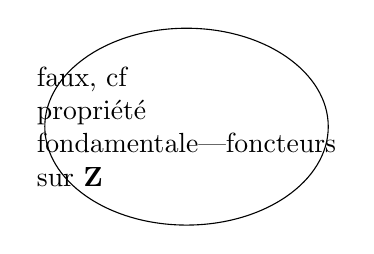
\begin{tikzpicture}
\draw (0,0) ellipse (1.8 and 1.25);
\node[align=left] at (0,0) {faux, cf\\\unsure{propriété}\\\unsure{fondamentale|foncteurs}\\sur $\mathbf Z$};
\end{tikzpicture}}}

Quant aux $\xi_{x,\mathbf C}=\xi_{x,\infty}$, eux \unsure{ms}
\deleted{\unsure{puisque}}\inserted{comme $k$ est}
\deleted{\unsure{nous avons dit}, ils sont}
alg. clos ils sont isomorphes entre eux, mais pas canoniquement ....

\uline{NB} En car $p>0$, je pense que $T_\alpha(\mathbf R)=\varnothing$
en général, ce qui explique qu'il n'y ait pas de phénomènes de
``composantes connexes'' ``Ramification en $\mathbf R$'' ...
à considérer alors ...

\margin{\unsure{s'éclaircir si} il ne peut y avoir des pt à val. dans une ext. tot. réelle ???}

Si

\figure{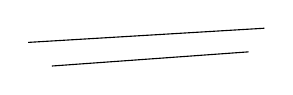
\begin{tikzpicture}\draw (0,0)--(3,.18);\draw (.3,-.3)--(2.8,-.12);\end{tikzpicture}}

Pt motivique de $X$ à valeurs dans un corps (ou un anneau) $k$: objet de $T(k)$.
Langage de la \uline{fibre d'un motif en un point}.
Les pts forment une catégorie fibrée sur $(\mathrm{Sch})$, munie de fpqc,
\deleted{\unsure{elle}} c'est un \uline{torseur}.
Pour $k$ donné, les isom. d'un \deleted{objet} $\xi\in T(k)$ sur un autre forment le

\margin{206}
\scanpage{208}
SYSTÈMES de RACINES (3) \hfill Tribu n$^\circ$ 59

linéaire réelle $\alpha\in\underline{a}^*$ sur $\underline{a}$, soit
$\underline{g}^\alpha=\{x\in\underline{g}\mid[a,x]=(a).x\ (a\in\underline{a})\}$.
Alors l'ensemble $R$ des éléments $\alpha\in\underline{a}^*-0$ pour lesquels
$\underline{g}^\alpha\ne(0)$ est un système de racines, en général non réduit.
Le groupe de Weyl de $R$ s'identifie au groupe des automorphismes de $\underline{a}$ induits par des éléments de $\operatorname{Ad}_{\underline{g}}\underline{k}$ laissant $\underline{a}$ stable.

III. Soient $k$ un corps, $G$ un groupe linéaire algébrique connexe semi-simple sur $k$, $T$ un tore algébrique sur $G$ décomposé sur $k$ maximal, et $X^*$ le groupe des caractères rationnels de $T$.
Le dual $X_*$ de $X^*$ s'identifie canoniquement au groupe des homomorphismes rationnels du groupe multiplicatif $G_m$ dans $T$.
Soit $\underline{g}$ l'algèbre de Lie de $G$ et, pour $\alpha\in X^*$, soit
$\underline{g}^\alpha=\{x\in\underline{g}\mid\operatorname{Ad}t(x)=\alpha(t).x\ (t\in T)\}$.
Alors l'ensemble $R$ des éléments non nuls $\alpha\in X^*$ pour lesquels $g^\alpha\ne(0)$ est un système de racines, qui est réduit si $T$ est aussi un sous-groupe de Cartan de $G$, ce qui a en particulier toujours lieu lorsque $k$ est algébriquement clos.
Le groupe de Weyl $W(R)$ s'identifie au quotient du normalisateur de $T$ par le centralisateur de $T$ dans $G$.

Si $k=\underline{C}$ l'algèbre de Lie $\underline{t}$ de $T$ est une sous-algèbre de Cartan de $\underline{g}$ et $R$ est isomorphe au système de racines défini en I.
Si $k=\underline{R}$, alors l'ensemble des points réels de $\underline{t}$ est conjugué à l'algèbre $\underline{a}$ considérée en II, et $R$ est isomorphe au système de racines défini en II.

IV. Soient $G$ un groupe de Lie compact connexe semi-simple, $\underline{g}$ son algèbre de Lie, $T$ un tore maximal de $G$ et $X$ le groupe des homomorphismes continus de $T$ dans $\underline{C}^*$.
Pour tout $\alpha\in X$, soit $\underline{g}^\alpha=\{x\in\underline{g}\mid\operatorname{Ad}t(x)=\alpha(t).x\ (t\in T)\}$.
Alors l'ensemble $R$ des éléments $\alpha\in X-0$ pour lesquels $\underline{g}^\alpha\ne(0)$ est un système de racines réduit dans $V=X\otimes\underline{Q}$, dont le groupe de Weyl s'identifie au quotient par $T$ du normalisateur de $T$ dans $G$.
On a $Q(R)\subset X\subset P(R)$ et $X=P(R)$, (resp. $X=Q(R)$), si $G$ est simplement connexe, (resp. isomorphe à $\operatorname{Ad}\underline{g}$). L'algèbre de

\margin{207}
\scanpage{209}
sch de \uline{classes de chemins}, ils sont déterminés \inserted{(s'il y en a au moins un)} par les automorphismes des foncteurs, qui font les pts d'un groupe algébrique.
Mais en général il peut y avoir des pts à valeurs dans un même $k$ non isomorphes.
Le groupe de Galois opérant sur \deleted{les points} l'ens des pts à valeurs dans $k$.
Si on a un pt $\xi$ à val. dans $k$, tous les autres pts s'en déduisent par des fibrés principaux \unsure{hom.} \unsure{du|au} (pro)groupe algébrique $\underline{\operatorname{Aut}}(\xi)$.

\diagram{\[
\left\{\begin{array}{ll}
\text{Pts $\ell$-adiques}&\text{valeurs }\mathbf Z_\ell\ \unsure{\text{ou}|-}\ \mathbf Q_\ell\\[6pt]
\text{Pts transcendants}&\text{valeurs }\mathbf R\ \deleted{\text{ou }\mathbf C\ \inserted{\unsure{\text{alg.}|\text{sup.}}}}\ \text{voire }\mathbf Z\\
&\begin{gathered}
\text{[structure supplémentaire]}\\
\text{Je doute que ces pts correspondent}\\
\text{biunivoquement aux pts de}\\
X\text{ à valeurs dans }\mathbf C,\\
\text{mod conjugaison}
\end{gathered}
\end{array}\right.
\]
\[
\begin{array}{ll}
\text{Pts Hodge-de Rham}&\text{valeur }k\text{ quelconque}\\
\text{pts de Witt}&\text{valeurs }W_p(k)\quad\text{$k$ corps de car $p$}
\end{array}
\]}

\margin{208}
\scanpage{210}
SYSTÈMES de RACINES (2) \hfill Tribu n$^\circ$ 59

Pour orienter le lecteur, nous indiquons ici les principaux exemples de systèmes de racines que l'on rencontre dans la théorie des groupes et algèbres de Lie.

I. Soient $\underline{g}$ une algèbre de Lie semi-simple sur $\underline{C}$ et $\underline{h}$ une sous-algèbre de Cartan de $\underline{g}$.
L'algèbre $\underline{h}$ est donc commutative, formée d'éléments semi-simples.
Une racine de $\underline{g}$ par rapport à $\underline{h}$ est une forme linéaire $\alpha$ non nulle sur $\underline{h}$ pour laquelle il existe $x\in\underline{g}$, $x\ne0$, tel que $[h,x]=\alpha(x)$ quel que soit $h\in\underline{h}$.
Soit $V$ l'espace vectoriel sur $\underline{Q}$ engendré par l'ensemble $R$ des racines de $\underline{g}$ par rapport à $\underline{h}$.
Alors $\underline{h}^*=V\otimes\underline{C}$, et $R$ est un système de racines réduit dans $V$, au sens du \S\ 6.
Tout système de racines réduit est l'ensemble des racines d'une algèbre semi-simple complexe, unique à son isomorphisme près.
Tout automorphisme de $\underline{g}$ laissant stable $\underline{h}$ induit un automorphisme de $\underline{h}^*$ laissant $R$ et $V$ invariants, et le groupe des automorphismes de $R$ ainsi obtenus à partir des automorphismes, (resp. des automorphismes intérieurs), de $\underline{g}$ s'identifie au groupe de tous les automorphismes de $R$, (resp. au groupe de Weyl de $R$).
Identifions le dual de $V$ à une $\underline{Q}$-forme $\underline{h}^0$ de $\underline{h}$ et soit $G$ un groupe de Lie complexe connexe d'algèbres de Lie $\underline{g}$.
Alors le noyau $\unsure{\Gamma|T}$ de l'application exponentielle de $\underline{h}$ dans $G$ est un réseau de $i.\underline{h}^0$ compris entre $2\pi i.Q(R^*)$ et $2\pi i.P(R^*)$, où $R^*$ est le système de racines inverse de $R$, qui est égal à $2\pi i.Q(R^*)$, (resp. $2\pi iP(R^*)$), si $G$ est simplement connexe, (resp. isomorphe à $\operatorname{Ad}\underline{g}$).
Le groupe $2\pi i.P(R^*)/\unsure{\Gamma|T}$ s'identifie au centre de $G$, et $\unsure{\Gamma|T}/2\pi i.Q(R^*)$ au groupe fondamental de $G$.
Le réseau de $V$ associé à $(2\pi i)^{-1}.\unsure{\Gamma|T}$ est engendré par les poids des représentations de $G$.

II. Soient $\underline{g}$ une algèbre de Lie semi-simple sur $\underline{R}$, $\underline{k}$ une sous-algèbre compacte maximale de $\underline{g}$, $\underline{p}$ le complément orthogonal de $\underline{k}$ par rapport à la forme de Killing, et $\underline{a}$ une sous-algèbre commutative maximale de $\underline{p}$. Pour toute forme

\margin{209}
\scanpage{211}
\margin{\figure{\begin{tikzpicture}
\node[rotate=52] at (0,0) {À revoir};
\draw (.8,7.5) .. controls (.65,3) and (1,-2) .. (.35,-8.5);
\end{tikzpicture}}}
\uline{Questions}

\diagram{\[
\left\{\begin{array}{l}
\left\{\begin{array}{l}
\text{pts \inserted{de $X$} à val. dans $k$ \inserted{de car $p>0$}: correspondent aux}\\
\text{pts motiviques \inserted{dans $W(k)$ (\unsure{ou|son} corps des fractions?)}}\\
\text{avec \uline{structure supplémentaire}}
\quad\figure{\begin{tikzpicture}[baseline=(fv.base)]
\node[draw,ellipse,inner sep=4pt] (fv) {$F\deleted{\unsure{F}},V$};
\end{tikzpicture}}
\quad\begin{gathered}\text{[foncteurs des}\\\text{groupes formels]}\end{gathered}\\
\begin{tikzcd}[column sep=12pt,row sep=5pt]
{}\arrow[rd,rightsquigarrow]&{}\\
{}&\begin{gathered}\text{pts motiviques généralisés}\\
\text{(au sens cat. \unsure{dérivées})}\\
\text{dans $k$, avec}\\\text{structure filtrée !}\end{gathered}
\end{tikzcd}
\end{array}\right.\\[14pt]
\begin{gathered}
\text{pts \inserted{de $X$} à val. dans $k$ de car 0: correspondent}\\
\text{aux pts motiviques dans $k$,}\\
\text{avec \uline{structure filtrée}}
\end{gathered}
\end{array}\right.
\]}

\diagram{\[
\left|\begin{array}{l}
\text{pts \inserted{de $X$} à valeurs dans $\mathbf C$ mod conj. complexes}\\
\begin{tikzcd}[column sep=12pt]
\text{(= place)}\arrow[r,leftrightarrow]&
\text{pts \inserted{motiviques} à valeurs dans }
\figure{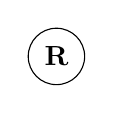
\begin{tikzpicture}[baseline=(r.base)]\node[draw,circle] (r) {$\mathbf R$};\end{tikzpicture}},\ \text{ou}
\end{tikzcd}\\
\text{à valeurs dans }
\figure{\begin{tikzpicture}[baseline=(cf.base)]
\node[draw,ellipse,inner sep=5pt] (cf) {$\mathbf C\text{ avec }f_\infty$};
\draw (.66,0) ellipse (.24 and .42);
\end{tikzpicture}},\ \text{ou}\\
\text{à valeurs dans }\mathbf Z
\end{array}\right.
\]}

\uline{\deleted{\unsure{Sch $X$ de}} car $p$}

\uline{Pts banaux}\quad Pts à valeurs dans
\figure{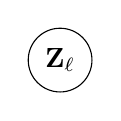
\begin{tikzpicture}[baseline=(zl.base)]\node[draw,circle] (zl) {$\mathbf Z_\ell$};\end{tikzpicture}},
$\ell$ premier aux car résiduelles.

\hfill ou
\figure{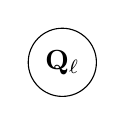
\begin{tikzpicture}[baseline=(ql.base)]\node[draw,circle] (ql) {$\mathbf Q_\ell$};\end{tikzpicture}}

\figure{\begin{tikzpicture}\draw[->] (0,1.2)--(0,0);\end{tikzpicture}}
\uline{Cas particulier important}\quad
\uline{Pts à valeurs dans corps} fini $\mathbf F_q$ correspondent aux pts à valeurs dans
\unsure{les|le}
\figure{\begin{tikzpicture}[baseline=(w.base)]\node[draw,ellipse] (w) {$W(\mathbf F_q)$};\end{tikzpicture}},
avec structure supplémentaire $(F,V)$

\margin{210}
\scanpage{212}
\hfill Tribu n$^\circ$ 59

\begin{center}SYSTÈMES de RACINES\end{center}

\begin{center}\uline{Introduction}, (Rédaction Borel).\end{center}

Ce chapitre est principalement consacré à l'étude de certains ensembles finis de vecteurs d'un espace euclidien, appelés systèmes de racines, et des groupes de déplacements d'un espace euclidien vectoriel ou affine engendré par des réflexions.
Son but est de fournir le cadre naturel dans lequel s'expriment et se démontrent un grand nombre de propriétés importantes des groupes et algèbres de Lie semi-simples sur $\underline{R}$ ou sur $\underline{C}$ et des groupes algébriques semi-simples sur un corps quelconque.
Bien que la rédaction ait été dictée par les besoins des chapitres suivants de ce Livre, nous avons été amenés en plusieurs endroits à élargir de diverses façons les hypothèses faites sur les groupes envisagés, de manière à placer certains résultats dans leur domaine naturel de validité, qui déborde parfois celui des applications que nous avons en vue.
Le lecteur uniquement intéressé à ces dernières peut concentrer son attention sur les systèmes de racines, (\S\ 6), et sur leurs groupes de Weyl vectoriels ou affines.
Il peut se limiter, dans le \S\ 1 aux réflexions d'un espace euclidien ou d'un $\underline{Z}$-module libre, dans le Théorème 1 du \S\ 7 à l'implication $(a)\Longrightarrow(b)$ lorsque $k=\underline{R}$ et que $G$ est engendré par des réflexions, et envisager la discussion des groupes de Coxeter faite au \S\ 4 avant tout comme un auxiliaire permettant de donner une démonstration unifiée des propriétés fondamentales des groupes de déplacements linéaires ou affines engendrés par des réflexions $^*$.

\figure{\begin{tikzpicture}\draw[dash pattern=on 3pt off 6pt] (0,0)--(13,0);\end{tikzpicture}}

($^*$) Pour rédiger ce paragraphe, nous avons largement utilisé des Notes de Séminaire, (non publiées), de Jacques Tits.

\margin{211}
\scanpage{213}
\uline{Groupe fondamental motivique discret}

Soit $\xi\in\mathbf T(\mathbf Z)$, on pose
\[
\begin{aligned}
\pi_1(X,\xi)&=\operatorname{Aut}(\xi).\\
&=G_\xi(\mathbf Z)
\end{aligned}
\]

\uline{N.B.} En vertu de Borel\inserted{-\unsure{Housh|Harish}}, il n'y a qu'un nb fini de $\xi\in T_\alpha(\mathbf Z)$ possible, pour $\alpha$ donné.
D'où un nb fini de \uline{groupes fondamentaux discrets}.
Sont-ils tous \unsure{associés} à des \deleted{\unsure{champs}} \unsure{places} ??

$\xi\in T_\alpha(k)$, $k$ un anneau

$M$ motif $\in\operatorname{Ob}\unsure{\mathfrak M_\alpha|\mathcal M_\alpha}$

$M_\xi$ fibre en $\xi$,\qquad $M_\xi=\xi(M)$
\[
\pi_1(X,\xi)_{\unsure{a|\alpha}}=\operatorname{Aut}(\xi),\qquad
G(X,\xi)=\underline{\operatorname{Aut}}(\xi)
\]
\deleted{$\unsure{G_\xi}$}
\[
\pi_1(X,\xi)_{\unsure{a|\alpha}}\simeq G(X,\xi)(k)
\]
Comparaison avec $\pi_1(X^{\unsure{\mathrm{tr}|\mathrm{tv}}},\unsure{\bar x|\xi})$ quand $\xi$ provient d'un \uline{pt} \unsure{en $a$} ....

\uline{Ex}. $X$ connexe sur $\mathbf C$, $\xi$ défini par un pt de $X$ à valeurs dans $\mathbf C$.
Le foncteur $\xi_{\mathbf C}\deleted{\unsure{\otimes}}$ a une structure \uline{filtrée}.
$\xi$ considéré comme foncteur à valeurs dans les modules sous $\pi_1(X,\xi)$ muni d'une \uline{structure de Hodge} est \unsure{pl.} fidèle ....

\margin{212}
\scanpage{214}
\begin{center}1 -- 49 --\end{center}\hfill n$^\circ$ 413

Soient $G$ et $H$ deux noyaux de groupe de classe $C^r$.
Un \uline{morphisme} $\psi$ de $G$ dans $H$ est une application de classe $C^r$ de $G$ dans $H$ satisfaisant aux conditions suivantes:

(a) $\psi(e_G)=e_H\qquad\psi(\theta_G(x))=\theta_H(\psi(x))$ pour tout $x\in G$;

(b) si $(x,y)\in\Omega(G)$, alors $(\psi(x),\psi(y))\in\Omega(H)$ et on a:
\[
m_H(\psi(x),\psi(y))=\psi(m_G(x,y))
\]
(autrement dit $\psi$ est une représentation pour les lois de composition non partout définies sur $G$ et $H$).
Nous laisserons au lecteur le soin d'étendre au cas des noyaux de groupe les propositions 3 et 3 bis.

Soit $G$ un noyau de groupe.
Il existe un voisinage ouvert $V$ de $e$ tel que les conditions de (iii) soient réalisées pour $x,y,z\in V$.
En particulier le \uline{produit de convolution} associé à la restriction de $m$ à $V\times V$ définit une loi de composition sur $T_e^{(r)}(G)$, qui est bilinéaire et associative (bien que non partout définie si $r<\infty$).
Nous désignerons encore par $U(G)$ l'espace $T_e^{(r)}(G)$ muni de cette multiplication.
Nous laisserons au lecteur le soin d'étendre les autres notations et résultats des n$^{\mathrm{os}}$ 12 à 16.
Signalons par exemple que si $f$ est un morphisme de $G$ dans un noyau de groupe $H$, alors $f_*$ est une \uline{représentation} de $U(G)$ dans $U(H)$.

De plus, l'application tangente $m^T$ à $m$ est une application de classe $C^{r-1}$ de $T(\qquad)$ dans $T(G)$.
On peut identifier $T(\qquad)$ à un ouvert de $T(G)\quad T(G)$ et on vérifie aisément que $T(G)$ muni du point marqué $0_e$, de l'application $m^T$ de $T(\qquad)$ dans $T(G)$ et de l'application $\theta^T$ de $T(G)$ dans $T(G)$ est un \uline{noyau de groupe} de classe $C^{r-1}$; la projection canonique est un morphisme de classe $C^{r-1}$ de $T(G)$ sur $G$.
Nous laisserons au lecteur le soin d'étendre au cas des noyaux de groupe les propositions 11 et 12 ainsi que leurs corollaires.

\margin{213}
\scanpage{215}
(Résulte de la \unsure{conjonction} des conj de Hodge et de Tate
\inserted{\figure{\begin{tikzpicture}[baseline=(n.base)]\node[draw,ellipse] (n) {sous forme faible};\end{tikzpicture}}},
du moins si $X$ \uline{connexe}).
\uline{\uuline{Caractériser \deleted{de} l'image}} ??

\margin{\figure{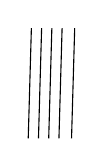
\begin{tikzpicture}\foreach \x in {0,.13,.26,.39,.55}{\draw (\x,0)--(\x+.04,1.4);}\end{tikzpicture}}}

\unsure{M} conclusion si $X$ défini sur $k\subset\mathbf C$, $k$ alg. clos, p.ex. $k=\overline{\mathbf Q}$.

\uline{Analyser l'exemple de Serre de $\pi_1$ non isomorphes}

[\uline{Cas corps de base} $\mathbf R$: tout pt \deleted{\unsure{réel}} \inserted{$a$} définit une $\xi_a\in T_\alpha(\mathbf Z)$.
Tous ces $\xi_a$ sont isomorphes \unsure{pour|puis} si \deleted{\unsure{a}} $X$ est
\deleted{\unsure{géom.} connexe, \unsure{sinon}}
\inserted{\unsure{irrid|irred} (pas néc. géom \unsure{irrid|irred})}
\deleted{il peut y en avoir deux non isom.}
\unsure{Si $a$} est un pt réel, alors $\xi_{\unsure{a|b}}$ \unsure{admet} un autom $\operatorname{frob}_\infty$ d'ordre 2, qui avec la comp. conn. de $G(X,\xi)$ engendre $G(X,\xi)$.

\margin{\diagram{\begin{tikzcd}[column sep=8pt,row sep=9pt]
&X\arrow[dl,no head]\arrow[dd,no head]\\
\mathbf C\arrow[dr,no head]&\\
&\mathbf R
\end{tikzcd}}}

Le foncteur
\[
M\mathrel{\unsure{\mapsto|\sim}}
(\unsure{\xi(M_\xi)|\xi(M)},+\text{structure de Hodge}+\text{involution définie par }\operatorname{frob}_\infty)
\]
est pleinement fidèle.]

\uline{Pb} étudier comment varie la structure de Hodge sur un pt \inserted{complexe} variable,
\uline{en fonction de} la \uline{donnée \unsure{départ}} en le pt $a_0$.

\margin{\figure{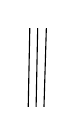
\begin{tikzpicture}\draw (0,0)--(.02,1);\draw (.1,0)--(.12,1);\draw (.2,0)--(.23,1);\end{tikzpicture}}}
\margin{214}
\scanpage{216}
\begin{center}1 -- 48 --\end{center}\hfill n$^\circ$ 413

17. \uline{Noyaux de groupe}.

DÉFINITION 5.-- \uline{On appelle noyau de classe} $C^r$ \uline{une variété} $V$ \uline{de classe} $C^r$ \uline{munie d'un point marqué} $e$.
\uline{Un noyau de groupe de classe} $C^r$ \uline{est un noyau} $G$ \uline{muni d'une application} $\theta_G$ \uline{de classe} $C^r$ \uline{de} $G$ \uline{dans} $G$ \uline{et d'une application} $m_G$ \uline{de classe} $C^r$ \uline{d'un ouvert} $\Omega(G)$ \uline{de} $G\times G$ \uline{dans} $G$ \uline{satisfaisant aux conditions suivantes}:

(i) $\Omega$ \uline{contient les points} $(x,\theta(x))$ \uline{et} $(\theta(x),x)$ \uline{et on a}
\[
\tag{36}m(x,\theta(x))=m(\theta(x),x)=e
\]
\uline{pour tout} $x\in G$;

(ii) $\Omega$ \uline{contient les points} $(e,x)$ \uline{et} $(x,e)$ \uline{et on a}
\[
\tag{37}m(e,x)=m(x,e)=x
\]
\uline{pour tout} $x\in G$;

(iii) \uline{si} $x,y,z$ \uline{sont trois éléments de} $G$ \uline{tels que} $(x,y)$, $(y,z)$, $(m(x,y),z)$ \uline{et} $m(x,m(y,z))$ \uline{appartiennent à} $\Omega$, \uline{on a}:
\[
\tag{38}m(m(x,y),z)=m(x,m(y,z)).
\]

On a $e=m(e,\theta(e))=\theta(e)$ et
\[
\begin{aligned}
x&=m(e,x)=m(m(\theta(\theta(x)),\theta(x)),x)=\\
&=m(\theta(\theta(x)),m(\theta(x),x)=m(\theta(\theta(x)),e)=\theta(\theta(x)).
\end{aligned}
\]

\uline{Exemple} 1.-- Une variété de groupe est un noyau de groupe.

\uline{Exemple} 2.-- Soient $X$ une variété, $e\in X$ et $m$ une application d'un ouvert $\Omega$ de $X\times X$ dans $X$ satisfaisant aux conditions (ii) et (iii) de la définition 5.
Le lemme 1 du n$^\circ$ 3 montre qu'il existe un voisinage ouvert $G$ de $e$ dans $X$ et un automorphisme $\theta$ de $G$ sur lui-même satisfaisant à (i).
Il suffit alors de prendre pour $\Omega(G)$ l'ensemble des $(x,y)\in(G\times G)\cap\Omega$ tels que $m(x,y)\in G$ et pour $m_G$ la restriction de $m$ à $\Omega(G)$ pour obtenir sur $G$ une structure de noyau de groupe.

\margin{215}
\scanpage{217}
Lien avec la variété des modules pour des motifs polarisés rigidifiés:
si \deleted{\unsure{le}} $\mathcal M$ est une telle variété modulaire, alors un morphisme
\diagram{\begin{tikzcd}[column sep=12pt]X\arrow[r,no head]&\mathcal M\end{tikzcd}}
est déterminé quand on connaît sa valeur \uline{en un point}, plus l'application
\diagram{\begin{tikzcd}[column sep=12pt]\pi_1(X)\arrow[r,no head]&\pi_1(\mathcal M)\end{tikzcd}}
......

C'est une propriété intrinsèque importante de ces $\mathcal M$, et une propriété de cette nature mérite d'être étudiée pour ses propres mérites .....
Peut-être peuvent elles \unsure{toutes} être
\deleted{\unsure{caractérisées}}\inserted{\unsure{interprétées}}
comme des \deleted{\unsure{schémas}}\inserted{variétés} modulaires pour certains types de motifs..

\figure{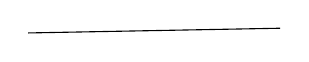
\begin{tikzpicture}\draw (0,0)--(3.2,.06);\end{tikzpicture}}

Introduire la notion de schéma \inserted{motiviquement} ponctué,
\inserted{\figure{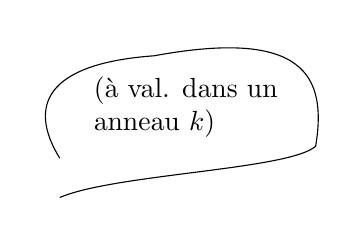
\begin{tikzpicture}[baseline=(a.base)]
\node[align=left] (a) {(\unsure{à val.} dans un\\anneau $k$)};
\draw (-1.6,-.65) .. controls (-2,0) and (-1.8,.55) .. (-.4,.65)
.. controls (1.5,1) and (1.8,.4) .. (1.65,-.5)
.. controls (1.3,-.8) and (-.9,-.85) .. (-1.6,-1.15);
\end{tikzpicture}}}
et morphismes de tels, qui définissent des morphismes correspondants pour les
\diagram{\begin{tikzcd}[column sep=16pt]G(X,\xi)\arrow[r,no head]&G(Y,\eta)\end{tikzcd}},
donc pour
\diagram{\begin{tikzcd}[column sep=18pt]
G(X,\xi)(k)=\pi_1(X,\xi)\arrow[r,no head]&G(Y,\eta)(k)=\pi_1(Y,\eta).
\end{tikzcd}}

\margin{216}
\scanpage{218}
\begin{center}1 -- 47 --\end{center}\hfill n$^\circ$ 413

16. \uline{Mesure de Haar d'une variété de groupe}.

Conservons les notations de la fin du n$^\circ$ précédent.
L'espace $\Omega_e^n(G)$ est alors de dimension 1 et il en résulte que \uline{l'espace des formes différentielles invariantes à gauche et de degré} $n=\dim G$ \uline{est de dimension} 1.
On en obtient une \uline{base} en prenant une base $\omega_1,\ldots,\omega_n$ de $\Omega_e^1(G)$ et en prenant le produit extérieur des formes $I_{\omega_k}^g$.
Avec les notations de (30), on obtient en prenant $\omega_k=dx_k$, l'expression d'une forme invariante à gauche $I_\omega^g$ de degré maximum au voisinage de $e$:
\[
\tag{31}I_\omega^g(x)=(\operatorname{dét}\partial m_k/\partial y_j(x^{-1};x))\,dx_1\cdots dx_n.
\]
D'autre part, il est clair que l'espace des formes différentielles invariantes à gauche est invariant par translations à droite.
Il existe donc une fonction de classe $C^{r-1}$ sur $G$, soit $\delta$, telle que:
\[
\tag{32}I_\omega^g(xy)=\delta(y)I_\omega^g\qquad(x,y\in G,\ \omega\in\Omega_e^n(G)).
\]
Mais on a $\delta(y)I_\omega^g=I_\omega^g(xy)=I_\omega^g(y^{-1}xy)=I_{\omega'}^g$ avec $\omega'=(\operatorname{ad}y^{-1})_*(\omega)$.
D'où:
\[
\tag{33}\delta(y)=(\operatorname{dét}\operatorname{ad}y)^{-1}.
\]

Supposons maintenant que $K$ soit \uline{localement compact} et soit $\omega\in\Omega_e^n(G)$.
Il est clair que la mesure $\mu=|I_\omega^g|$ est une \uline{mesure de Haar à gauche} sur le groupe localement compact $G$.
Avec les notations de (30) et (31), on a donc pour $x$ voisin de $e$:
\[
\tag{34}d\mu(x)=\operatorname{mod}(\operatorname{dét}\partial m_k/\partial y_j(x^{-1};x))\,dx_1\cdots dx_n
\]
où mod est le \uline{module} du corps localement compact $K$ (Int. VII, \S\ 1, n$^\circ$ 10 et F. R. V.).
D'autre part, (32) et (33) montrent que le \uline{module} du groupe localement compact $G$ (Int. VII, \S\ 1, n$^\circ$ 3, déf. 3) n'est autre que
\[
\tag{35}\Delta(y)=\operatorname{mod}(\delta(y))=\operatorname{mod}(\operatorname{dét}\operatorname{ad}y)^{-1}.
\]

\margin{217}
\scanpage{219}
$X$ \deleted{schéma} préschéma de type fini \inserted{normal} irréductible sur corps $k$

$\unsure{v|\nu},\unsure{w|\omega}$ deux places archimédiennes de \deleted{\unsure{le}} $X$, d'où foncteurs fibres
$\xi_{\unsure{v|\nu}}^{\mathbf Z},\xi_{\unsure{w|\omega}}^{\mathbf Z}$.
Question: a) \inserted{Quand} sont-ils isomorphes?
b) \deleted{Est-il vrai que} Quand est-il vrai que pour tte sous-catégorie \inserted{mult.} de t.f. de $\mathcal M(X)$, les restrictions de ces foncteurs à $\mathcal M_\alpha(X)$ sont isomorphes?

Nous pouvons supposer, quitte à remplacer $k$ par
\deleted{\unsure{Soient $v',w'$ les}}
sa clôture alg. dans $k(X)$, que $k$ est alg. clos dans $k(X)$ [\unsure{utilise|utiliser} le fait $X$ \uline{normal}!]
donc $X$ est géom\textsuperscript{t} \unsure{irrid.|irred.} sur $k$.
Soit \deleted{$k_0$} \inserted{$k_0$ la clôture alg. de $\mathbf Q$ dans $k$.}
\deleted{le corps des \unsure{coïncidences} des places (= val. abs.) induites sur $k$, \unsure{envisagées}}
\inserted{\uline{contient la clôture alg. $\unsure{E}$ de $\mathbf Q$ dans $k$} (p.ex. $k_0$ alg. fermé dans $k$).}
\deleted{1) $k_0$ est algébriquement fermé dans $k$. Alors}
\inserted{1°) $\unsure{v|\nu},\unsure{w|\omega}$ coïncident sur $k_0$.}

\[
\text{a)}\quad \xi_{\unsure{v|\nu}}^{\mathbf Z}|\mathcal M_\alpha(X)
\simeq \xi_{\unsure{w|\omega}}^{\mathbf Z}|\mathcal M_\alpha(X)
\quad\text{pour }\forall\ \alpha.
\]

\margin{\diagram{\begin{tikzcd}[column sep=13pt,row sep=12pt]
&X_0\arrow[r,no head]\arrow[d,no head]&X\arrow[d,no head]\\
k_0\arrow[r,no head]&A_0\arrow[r,no head]&k
\end{tikzcd}}}

En effet, $X$ et $\mathcal M_\alpha(X)$ proviennent de $X_0$, \inserted{$\mathcal M_\alpha(X_0)$}, de type fini sur $A_0$, \inserted{$k_0$}$k$-alg. de type fini de $k$,
\deleted{$X_0\longrightarrow\operatorname{Spec}A_0$ fid plt \unsure{et irred sur} $A_0$}\inserted{\unsure{conn et}} $^*$
\deleted{\unsure{et}}
On est ramené au cas où $k=\unsure{k_0|E_0}$, où on obtient le résultat voulu grâce au groupe fondamental transcendant.

\margin{\deleted{\diagram{\begin{tikzcd}[column sep=12pt,row sep=10pt]
&\unsure{X_0}\arrow[r,no head]\arrow[d,no head]&X\arrow[d,no head]\\
E\arrow[r,no head]\arrow[dr]&\unsure{k_0}\arrow[r,no head]\arrow[d,no head]&k\\
& A_0\arrow[r,no head]&\unsure{E|\mathbf Z}\\
&\unsure{\mathbf Q}\arrow[u,no head]\arrow[ur,no head]&
\end{tikzcd}}}}

\deleted{\unsure{Alors}}
b) Si \deleted{$k=k_0$}\inserted{$\unsure{v|\nu}$ et $\unsure{w|\omega}$ coïncident sur $k$,}
cet argument montre que
$\xi_{\unsure{v|\nu}}^{\mathbf Z}\simeq\xi_{\unsure{w|\omega}}^{\mathbf Z}$.
\inserted{sinon, mais \unsure{si on suppose} $k$ est \illegible{1}}
\deleted{Si $k\ne k_0$, \unsure{on peut} $\xi_{\unsure{v|\nu}}^{\mathbf Z}\ne\xi_{\unsure{w|\omega}}^{\mathbf Z}$, \unsure{géom} \illegible{1}}

\margin{$^*$ on peut supposer $X_0\to\operatorname{Spec}A_0$ fid plt \unsure{géomt connexe}, et
\diagram{\begin{tikzcd}[column sep=8pt]\operatorname{Spec}(A_0)\arrow[r,no head]&k_0\end{tikzcd}}
géom connexe, donc
\diagram{\begin{tikzcd}[column sep=8pt]X_0\arrow[r,no head]&\operatorname{Spec}k_0\end{tikzcd}}
géom connexe.}
\figure{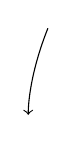
\begin{tikzpicture}\draw[->] (0,1.1) .. controls (-.2,.6) and (-.25,.2) .. (-.25,0);\end{tikzpicture}}

\margin{218}
\scanpage{220}
\begin{center}-- 12 --\end{center}\hfill n$^\circ$370

4) Supposons $G$ unimodulaire. Soit $\mu$ une mesure de Haar sur $G$. On a
\[
\tag{26}\gamma(s)\mu=\delta(s)\mu=\check\mu=\mu.
\]
Si $f$ est $\mu$-intégrable sur $G$, les translatées à gauche et à droite de $f$ sont $\mu$-intégrables ainsi que $\check f$, et on a
\[
\tag{27}\int f(sx)d\mu(x)=\int f(xs)d\mu(x)=\int f(x^{-1})d\mu(x)=\int f(x)d\mu(x).
\]
Si $A$ est une partie $\mu$-intégrable de $G$, $sA$, $As$ et $A^{-1}$ sont $\mu$-intégrables, et
\[
\tag{28}\mu(sA)=\mu(As)=\mu(A^{-1})=\mu(A).
\]
On a des propriétés analogues pour l'intégrale essentielle.

PROPOSITION 2.-- \uline{S'il existe dans} $G$ \uline{un voisinage compact} $V$ \uline{de} $e$ \uline{invariant par automorphismes intérieurs}, \uline{alors} $G$ \uline{est unimodulaire}.

En effet, soit $\mu$ une mesure de Haar à gauche sur $G$.
On a, pour tout $s\in G$,
$\mu(V)=\mu(s^{-1}Vs)=\Delta_G(s)\mu(V)$, d'où $\Delta_G(s)=1$ puisque $0<\mu(V)<+\infty$.

On en déduit aussitôt:

COROLLAIRE.-- \uline{Si} $G$ \uline{est discret}, \uline{ou compact}, \uline{ou commutatif}, $G$ \uline{est unimodulaire}.

Ceci est d'ailleurs trivial lorsque $G$ est \uline{commutatif}.
Notons aussi que, si $G$ est \uline{discret}, la mesure sur $G$ pour laquelle chaque point est de masse 1 est évidemment une mesure de Haar à gauche et à droite sur $G$, qu'on appelle mesure de Haar \uline{normalisée} sur $G$.
Si $G$ est \uline{compact}, il existe une mesure de Haar $\mu$ et une seule sur $G$ telle que $\mu(G)=1$; on l'appelle la mesure de Haar \uline{normalisée} de $G$.
Les deux conventions précédentes ne concordent pas lorsque $G$ est à la fois discret et compact, c'est-à-dire fini; quand on sera dans ce cas, on précisera toujours explicitement ce qu'on entend par mesure de Haar normalisée.

Un sous-groupe, un groupe quotient d'un groupe unimodulaire ne sont pas toujours unimodulaires (\S\ 2, exerc. 5). Cf., toutefois, le \S\ 2, prop. 10.

$^*$Nous verrons plus tard que les groupes de Lie connexes semi-simples ou nilpotents sont unimodulaires.$^*$

\margin{219}
\scanpage{221}
\inserted{dénombrable (p.ex. de t.f. sur $\mathbf Q$)}
\deleted{un \uline{\unsure{suite|corps}} de \unsure{puissance}}, on voit encore que
$\xi_{\unsure{v|\nu}}^{\mathbf Z}\simeq\xi_{\unsure{w|\omega}}^{\mathbf Z}$.
En effet, $k$ est réunion filtrante d’une \uline{suite} $A_i$ de sous-$k_0$-algèbres de type fini,
on peut supposer les morphismes de transition
$\operatorname{Spec}A_j\mathbin{—}\operatorname{Spec}A_i$
lisses à fibres géom. connexes, donc idem pour $X_j\mathbin{—}X_i$,
donc aussi pour $X_{j\mathbf C}\mathbin{—}X_{i\mathbf C}$.
On a des pts $x_i,y_i$ dans $X_{i\mathbf C}$, s’envoyant les uns sur les autres par les
morphismes de transition, et grâce à la lissité et la connexité des fibres,
on voit que les morphismes de transition
$\pi^1(x_j,y_j)\mathbin{—}\pi^1(x_i,y_i)$ sont surjectifs.
Donc $\varprojlim_i\pi^1(x_i,y_i)\ne\varnothing$, on gagne.
\figure{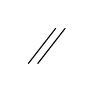
\begin{tikzpicture}\draw (0,0)--(.35,.45);\draw (.12,0)--(.47,.45);\end{tikzpicture}}
Si $k$ pas dénombrable,

2) \deleted{$E\subset k_0$ alg. fermé dans $k$.}
\inserted{$\unsure{v|\nu}$ et $\unsure{w|\omega}$ ne coïncident pas sur $E$.}
Alors je \deleted{\unsure{dis}}\inserted{pense} qu’il existe $\alpha$ tel que
\deleted{\unsure{et un motif} $M$,}
\[
 \xi_{\unsure{v|\nu}}^{\mathbf Z}|\mathcal M_\alpha(X)
 \not\simeq
 \xi_{\unsure{w|\omega}}^{\mathbf Z}|\mathcal M_\alpha(X).
\]
\margin{\deleted{$\unsure{\xi_v(M)}\ne\unsure{\xi_w(M)}$}}
On peut supposer que $X=\operatorname{Spec}\unsure{k|E}$, $k$ extension finie de $\mathbf Q$,
\deleted{\unsure{De plus}, \unsure{on peut supposer}, \unsure{pour} \illegible{4},
\unsure{que} $k$ \unsure{est} \illegible{1} \unsure{sur} $\mathbf Q$,}
\margin{220}
\scanpage{222}
\margin{221}
\begin{center}-- 9 --\end{center}
\margin{n$^\circ$370}
$\mu(f')\ne0$, on a $\mu((D_f-D_{f'})g)=0$ quelle que soit $g\in\mathcal K$ ;
remplaçant $g$ par $(D_f-D_{f'})g$, on obtient
$\mu((D_f-D_{f'})^2g)=0$ quelle que soit $g\in\mathcal K^+$,
donc $D_f=D_{f'}$ puisque le support de $\mu$ est $G$.
Posons donc $D_f=D$. La formule (14) donne
\[
(17)\qquad \mu(f)D(e)=\check\nu(f).
\]
La formule (17) s’étend par linéarité aux $f\in\mathcal K$ telles que $\mu(f)=0$.
On a $D(e)\ne0$ puisque $\check\nu\ne0$.
Ceci établit bien la proportionnalité de $\mu$ et $\check\nu$.

COROLLAIRE. -- \uline{Toute mesure complexe invariante à gauche}
(resp. \uline{à droite}) \uline{sur} $G$
\uline{est proportionnelle à une mesure de Haar à gauche}
(resp. \uline{à droite}).

\uline{Exemple} 1. -- Sur le groupe additif $\mathbb R$, la mesure de Lebesgue $dx$
est une mesure de Haar (Chap. III, § 2, n$^\circ$2, exemple).

\uline{Exemple} 2. -- Pour toute fonction $f\in\mathcal K(\mathbb R_+^*)$,
on a (Fonct. var. réelles, chap. II, § 1, formule (13))
\[
\int_0^{+\infty}\frac{f(x)}x\,dx
=\int_0^{+\infty}\frac{f(tx)}{tx}\,t\,dx
=\int_0^{+\infty}\frac{f(tx)}x\,dx
\]
quel que soit $t>0$ ; la mesure $x^{-1}dx$ est donc une mesure de Haar
sur le groupe multiplicatif $\mathbb R_+^*$.

\uline{Exemple} 3. -- Prenons pour $G$ le tore $\mathbb T=\mathbb R/\mathbb Z$.
Soit $\varphi$ l’application canonique de $\mathbb R$ sur $\mathbb T$.
Pour $f\in\mathcal K(\mathbb T)$, la fonction $f\circ\varphi$ est continue et
périodique de période 1 sur $\mathbb R$, et l’intégrale
$I(f)=\int_a^{a+1}f(\varphi(x))dx$ est indépendante du choix de $a\in\mathbb R$ ;
il est immédiat qu’elle est invariante par translation ; elle définit donc
une mesure de Haar sur $\mathbb T$. Par transport de structure, on en déduit que
$I(f)=\int_a^{a+1}f(e^{2\pi it})dt$ est une mesure de Haar sur le groupe
multiplicatif $\mathbb U$ des nombres complexes de valeur absolue 1
(Top. géné., chap. VIII, § 2, n$^\circ$1).

PROPOSITION 1. -- \uline{Soient} $G$ \uline{un groupe localement compact},
$\mu$ \uline{une mesure de Haar à gauche ou à droite sur} $G$.
\uline{Pour que} $G$ \uline{soit discret}, \uline{il faut et il suffit que}
\scanpage{223}
Il suffirait de construire $X$ projectif lisse sur $k$, tel que
$H^*(X_{\unsure{v|\nu}},\mathbf Z)$ et $H^*(X_{\unsure{w|\omega}},\mathbf Z)$
non isomorphes comme \uline{anneaux}.
On devrait mettre Serre à contribution.
\margin{Peut-on remplacer $\mathbf Z$ par $\mathbf R$ ??}
\figure{\begin{tikzpicture}\draw (0,0)--(2.5,0);\draw (.6,-.16)--(2,-.16);\end{tikzpicture}}

Soit $k$ un corps de nbs, $v_0$ une place de $k$, $M$ un motif sur $k$,
d’où $G_{Mv_0}=G_{v_0}$ grp algébrique \uline{défini sur} $\mathbf Z$.
Toute autre place \deleted{\unsure{de}} $v$ définit un fibré principal homogène
$P_v$ sous $G_{v_0}$,
\unsure{A} si on admet ce qui a été \deleted{dit}\inserted{conjecturé} plus haut,
\inserted{si $M$ est pris assez grand,}
\[
v\ne v'\Longrightarrow P_v\not\simeq P_{v'}.
\]
On peut aller plus loin et se demander si \deleted{\unsure{en}}
(pour $M$ assez grand) \uline{tt} fibré principal homogène $P$ sur $G_{v_0}$
provient d’une place $v$ \deleted{\unsure{complexe}}.
\figure{\begin{tikzpicture}\draw (0,0)--(.4,.6);\end{tikzpicture}}
\deleted{\unsure{les}} On \deleted{de} peut poser
\[
G_{Mv_{\unsure{0|a}}}(\mathbf Z)=\pi^1_M(k,v)
\]
\unsure{ces groupes} : \unsure{puis on est} \unsure{pour} \unsure{donner}
\unsure{nom} : groupes \uline{fondamentaux \inserted{(arithmétiques)} discrets}.
\margin{\figure{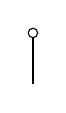
\begin{tikzpicture}\draw (0,0)--(0,.6);\draw (0,.65) circle (.06);\end{tikzpicture}}
Attention, la condition d’avoir un isomorphisme de foncteurs
$\xi(\unsure{N|M})\otimes_{\mathbf Z}\mathbf C\simeq M_\infty\otimes_k\mathbf C$,
satisfaisant aux conditions de compatibilité genre Riemann--Hodge,
risque d’être une condition \unsure{véritable sélection|véritable de sélection}....}
\figure{\begin{tikzpicture}\draw[->] (2,0)--(0,0);\end{tikzpicture}}
\margin{222}
\scanpage{224}
\margin{223}
\begin{center}-- 7 --\end{center}
\margin{n$^\circ$370}
si $f\le\sum_{i=1}^n c_i\gamma(s_i)g$ avec des $c_i\ge0$,
on a $\sup f\le\sum_{i=1}^n c_i g(s_i^{-1}s)$ pour un $s\in G$,
donc $\sup f\le(\sum_{i=1}^n c_i)\sup g$, d’où (iv).
Prouvons (v) ; soient $f\in\mathcal K$, $g,h\in\mathcal K_+^*$ ;
si $f\le\sum_{i=1}^n c_i\gamma(s_i)g$ et
$g\le\sum_{j=1}^p d_j\gamma(t_j)h$ ($c_i,d_j\ge0$, $s_i,t_j\in G$),
$f\le\sum_{i,j}c_i d_j\gamma(s_i t_j)h$, donc
$(f:h)\le\sum_{i,j}c_i d_j=(\sum_i c_i)(\sum_j d_j)$ ;
donc $(f:h)\le(f:g)(g:h)$.
Si on applique (v) à $f_0,f,g$ d’une part et à $f,f_0,g$ d’autre part,
on obtient (vi). Enfin, soient $f,f',h\in\mathcal K_+$ avec $h(s)\ge1$
sur le support de $f+f'$, et soit $\varepsilon>0$.
Posons $F=f+f'+\frac12\varepsilon h$ ; les fonctions $\varphi,\varphi'$,
qui coïncident respectivement avec $f/F$ et $f'/F$ sur le support de $f+f'$
et qui sont nulles en dehors de celui-ci, appartiennent à $\mathcal K_+$ ;
pour tout $\eta>0$, il existe un voisinage compact $V$ de $e$ tel que
$|\varphi(s)-\varphi(t)|\le\eta$ et $|\varphi'(s)-\varphi'(t)|\le\eta$
pour $s^{-1}t\in V$. Soit alors $g\in\mathcal K_+^*(V)$ ; pour tout $s\in G$,
on a $\varphi.\gamma(s)g\le(\varphi(s)+\eta).\gamma(s)g$
(en effet, c’est évident aux points où $\gamma(s)g$ s’annule, donc hors de $sV$ ;
et, dans $sV$, $\varphi\le\varphi(s)+\eta$) ; de même,
$\varphi'.\gamma(s)g\le(\varphi'(s)+\eta).\gamma(s)g$.
Ceci posé, soient $c_1,\ldots,c_n$ des nombres $\ge0$ et
$s_1,\ldots,s_n$ des éléments de $G$ tels que
$F\le\sum_{i=1}^n c_i\gamma(s_i)g$ ; on a
\[
f=\varphi F\le\sum_{i=1}^n c_i\varphi.\gamma(s_i)g
\le\sum_{i=1}^n c_i(\varphi(s_i)+\eta).\gamma(s_i)g
\]
et de même pour $f'$ ; par suite
\[
(f:g)+(f':g)\le\sum_{i=1}^n c_i(\varphi(s_i)+\varphi'(s_i)+2\eta)
\le(1+2\eta)\sum_{i=1}^n c_i
\]
puisque $\varphi+\varphi'\le1$. En appliquant la définition de $F$,
puis (ii), (iii), et (v), on en conclut
\[
\begin{aligned}
(f:g)+(f':g)&\le(1+2\eta)(F:g)
\le(1+2\eta)\bigl[(f+f':g)+\tfrac12\varepsilon(h:g)\bigr]\le{}\\
&\le(f+f':g)+\tfrac12\varepsilon(h:g)
+2\eta(f+f':h)(h:g)+\varepsilon\eta(h:g)
\end{aligned}
\]
et, si on a choisi $\eta$ tel que
$\eta[2(f+f':h)+\varepsilon]\le\frac12\varepsilon$, on obtient (vii).

Quand $V$ parcourt l’ensemble des voisinages compacts de $e$, les
$\mathcal K_+^*(V)$ forment une base de filtre $\mathcal B$ sur $\mathcal K_+^*$.
Soit $\mathcal F$ un ultrafiltre sur $\mathcal K_+^*$ plus fin que $\mathcal B$.
\scanpage{225}
\margin{\deleted{1 \unsure{cas initial} $X$ \unsure{du type} \illegible{2} \unsure{corps de base}}}
On a vu plus haut qu’une place est \unsure{trs|très} loin d’être caractérisée par le
foncteur fibre correspondant, \deleted{\unsure{le}}
considéré comme foncteur dans les $\mathbf Z$-modules.
Mais que se passe-t-il si on le regarde comme foncteur dans les structures de Hodge ?
\deleted{\unsure{Ceci devrait être} \unsure{disons que}}
\inserted{Vrai par un théorème \unsure{Rauch}, et par \illegible{1}}

\deleted{\unsure{par ailleurs le point}, on est \unsure{ramené} au cas où
\unsure{deux} \illegible{4} sur $k_0=$ clôture alg. de $\mathbf Q$ dans $k$,
et \unsure{puisqu’on a} $X$ est de type
$X$ est de type fini sur \deleted{\unsure{un}} $\mathbf Q$,
puis par changement de base on \unsure{a} $X$ est connexe de type fini sur $\mathbf C$,
et qu’on a deux pts \inserted{ordinaires} de $X$ à val. dans $\mathbf C$.
Supposons pour simplifier que \deleted{\unsure{tt}} $X$ est
\deleted{affine}, \inserted{(quasi-projectif)},
\unsure{voire affine}, \unsure{commençons par un cas simple} $X=\mathbf P^1_{\mathbf C}$.}

\margin{Attention, il faut partir de pts complexes, \unsure{non seulement de}
places, pour pouvoir définir la structure de Hodge.
\diagram{\begin{tikzcd}[column sep=small,row sep=small]
 & X \arrow[dl,no head] \arrow[dr,no head] & \\
 \unsure{\mathbf Q} \arrow[rr,no head] && k
\end{tikzcd}}
\deleted{$\unsure{A_i}$}
\figure{\begin{tikzpicture}\node at (0,.8) {$X$};\draw (0,.55)--(0,0);\end{tikzpicture}}}

Il semble qu’on le vérifiera facilement dans le cas de
$X=\mathbf P^1_{\mathbf C}-(0)-(1)-(\infty)$,
\inserted{(et deux pts à val. dans $\mathbf C$ \unsure{ord.})},
où les théorèmes classiques \deleted{\unsure{dit}} le donnent ---
[prendre comme motif celui défini par un schéma en courbes elliptiques sur $X$,
d’invariant l’indéterminée $j$].
\margin{224}
\scanpage{226}
\margin{225}
\begin{center}-- 6 --\end{center}
\margin{n$^\circ$370}
2. \uline{Le théorème d’existence et d’unicité}.

DÉFINITION 2. -- \uline{Soit} $G$ \uline{un groupe localement compact}.
\uline{On appelle mesure de Haar à gauche} (resp. \uline{à droite})
\uline{sur} $G$ \uline{une mesure positive non nulle sur} $G$,
\uline{invariante à gauche} (resp. \uline{à droite}).

THÉORÈME 1. -- \uline{Sur tout groupe localement compact},
\uline{il existe une mesure de Haar à gauche} (resp. \uline{à droite}),
\uline{et}, \uline{à un facteur constant près}, \uline{il n’en existe qu’une}.

A) \uline{Existence} -- Posons $\mathcal K(G)=\mathcal K$,
$\mathcal K_+(G)=\mathcal K_+$, $\mathcal K_+^*=\mathcal K_+-\{0\}$.
Si $C$ est une partie compacte de $G$, on notera $\mathcal K_+^*(C)$
l’ensemble des $f\in\mathcal K_+^*$ à support dans $C$.
Pour $f\in\mathcal K$ et $g\in\mathcal K_+^*$, il existe des nombres
$c_1,\ldots,c_n\ge0$ et des éléments $s_1,\ldots,s_n$ de $G$ tels que
$f\le\sum_{i=1}^n c_i\gamma(s_i)g$.
(En effet, il existe une partie ouverte non vide $U$ de $G$ telle que
$\inf_{s\in U}g(s)>0$, et le support de $f$ peut être recouvert par un nombre
fini de translatés à gauche de $U$).
Soit alors $(f:g)$ la borne inférieure des nombres $\sum_{i=1}^n c_i$
pour tous les systèmes $(c_1,\ldots,c_n,s_1,\ldots,s_n)$ de nombres $\ge0$
et d’éléments de $G$ tels que $f\le\sum_{i=1}^n c_i\gamma(s_i)g$.
On a :
\[
\begin{array}{lll}
\text{(i)} & (\gamma(s)f:g)=(f:g) & \text{pour }f\in\mathcal K,\ g\in\mathcal K_+^*,\ s\in G\ ;\\
\text{(ii)} & (\lambda f:g)=\lambda(f:g) & \text{pour }f\in\mathcal K,\ g\in\mathcal K_+^*,\ \lambda\ge0\ ;\\
\text{(iii)} & (f+f':g)\le(f:g)+(f':g) & \text{pour }f,f'\in\mathcal K,\ g\in\mathcal K_+^*\ ;\\
\text{(iv)} & (f:g)\ge(\sup f)/(\sup g) & \text{pour }f\in\mathcal K,\ g\in\mathcal K_+^*\ ;\\
\text{(v)} & (f:h)\le(f:g)(g:h) & \text{pour }f\in\mathcal K,\ g,h\in\mathcal K_+^*\ ;\\
\text{(vi)} & 0<\dfrac1{(f_0:f)}\le\dfrac{(f:g)}{(f_0:g)}\le(f:f_0)
& \text{pour }f,f_0,g\in\mathcal K_+^*\ ;
\end{array}
\]
(vii) soient $f,f',h\in\mathcal K_+$ avec $h(s)\ge1$ sur le support de $f+f'$,
et soit $\varepsilon>0$ ; il existe un voisinage compact $V$ de $e$ tel que,
pour toute $g\in\mathcal K_+^*(V)$, on ait
$(f:g)+(f':g)\le(f+f':g)+\varepsilon(h:g)$.

Les propriétés (i), (ii), (iii) sont évidentes.
Soient $f\in\mathcal K$, $g\in\mathcal K_+^*$ ;
\scanpage{227}
\margin{\figure{\begin{tikzpicture}\draw (0,.65)--(0,.12);\draw (0,.08) circle (.07);\end{tikzpicture}}
en vertu de la conjecture de Hodge}
D’autre part, \uline{quels} sont les foncteurs multiplicatifs de Motifs,
à valeurs dans les structures de Hodge,
\inserted{(i.e. \unsure{dans} les motifs sur $\mathbf C$ !)}
qui sont associés à des places archimédiennes ?
Plus généralement, dans quelle mesure un morphisme de préschémas
\inserted{$X\mathbin{—}Y$} est connu par le foncteur sur les motifs
\inserted{(loc. cit.)}, et dans quelle mesure un foncteur
\inserted{multiplicatif} peut-il être pris arbitrairement ???

C’est lié au Pb de \uline{construction des schémas de modules} pour les motifs
polarisés ; \unsure{si $M$} polarisé fidèle tel que
\inserted{($Y$ schéma sur \unsure{c. alg.})}
$Y\longrightarrow\mathrm{Modules}$ est une immersion
\inserted{(\unsure{resp. une}})
\deleted{\unsure{est}} alors \unsure{est|ça} \unsure{analogue}.
Kif kif si $Y$ est \uline{l’un} des préschémas ayant cette belle propriété.
Marchera en particulier si $Y$ est le spectre d’un corps.....
\margin{226}
\scanpage{228}
\margin{227}
\begin{center}-- 5 --\end{center}
\margin{n$^\circ$370}
On définit de manière analogue les mesures invariantes, relativement invariantes
et quasi-invariantes par $G$ sur $X$. Si $\mu$ est relativement invariante,
on définit son multiplicateur $\chi$ par les formules
\[
\begin{array}{ll}
(7') & \delta(s)\mu=\chi(s)\mu\\
(8') & \displaystyle\int_X f(xs)d\mu(x)=\chi(s)^{-1}\int_X f(x)d\mu(x)\\
(9') & \mu(As)=\chi(s)\mu(A).
\end{array}
\]
Si on considère le groupe opposé $G^o$ à $G$ comme opérant dans $X$ par
$(x,s)\longrightarrow xs$, $\mu$ est relativement invariante par $G^o$
de même multiplicateur $\chi$.

Soit enfin $G$ un groupe localement compact. Il opère sur lui-même par translations
à gauche et à droite, suivant les formules $\gamma(s)x=sx$, $\delta(s)x=xs^{-1}$.
Tout ce qui précède est applicable, et on a donc, sur $G$, les notions de mesures
\uline{invariantes à gauche}, \uline{invariantes à droite},
\uline{relativement invariantes à gauche}, \uline{relativement invariantes à droite},
\uline{quasi-invariantes à gauche}, \uline{quasi-invariantes à droite}
(cf., toutefois, les n$^{os}$ 6 et 9).

L’application $x\longrightarrow x^{-1}$ est un homéomorphisme de $G$ sur $G$.
Pour toute fonction $f$ sur $G$, on définira la fonction $\check f$ sur $G$ par
\[
(10)\qquad\check f(x)=f(x^{-1}).
\]
Pour toute mesure $\mu$ sur $G$, on définira la mesure $\check\mu$ par
\[
(11)\qquad\check\mu(f)=\mu(\check f)\qquad\text{pour }f\in\mathcal K(G).
\]
Autrement dit
\[
(12)\qquad\int_G f(x)d\check\mu(x)=\int_G f(x^{-1})d\mu(x)
\]
Si $A$ est un ensemble $\check\mu$-intégrable, $A^{-1}$ est $\mu$-intégrable, et
\[
(13)\qquad\check\mu(A)=\mu(A^{-1}).
\]
\cotefile{18}
\scanpage{2}
Papiers donnés à \unsure{Saavedra}
\margin{1}
\scanpage{3}
Page 6

Proposal to National Science Foundation

7. The Existence and Unicity of Best Approximations (with E.W. Cheney),
\uline{Math. Scand.}, (To Appear, Summer 1969).

8. Convergence of Operators and Korovkin’s Theorem.
\uline{J. of Approx. Theory}, \uline{1}, (1968), pp. 381--390.

9. Continuous Selections for Metric Projections (with A.J. Lazar and P.D. Morris),
\uline{J. of Funct. Analy.}, \uline{3}, (1968), pp. 193--216.

10. A characterization of $C(X)$ for $X$ locally connected.
\uline{Proc. Amer. Math. Soc.}, \uline{21}, (1969), pp. 269--272.

11. On the Minimal Property of the Fourier Projection
(with E.W. Cheney, C.R. Hobby, P.D. Morris and F. Schurer),
\uline{Trans. Amer. Math. Soc.}, (To Appear).

12. The classification of Banach spaces whose duals are $L_1$ spaces
(with J. Lindenstrauss). \uline{J. of Funct. Analy.}, (To Appear).

13. In Preparation. ``Characterizations of Conditional Expectations.''

RESEARCH ANNOUNCEMENTS

14. Structure of Tchebychev sets,
\uline{Proc. of the Second Symposium on General Topology and its Applications to Modern Analysis and Algebra},
Prague, 1966, pp. 356--359. This paper is an announcement of (4) above.

15. Locally connected Stone-Cech compactifications,
\uline{Proc. of First International Symposium on Extension Theory of Topological Structures and its Applications}
(To Appear). This paper is an announcement of (10) above.

16. On the minimal property of the Fourier Projection
(with E.W. Cheney, C.R. Hobby, P.D. Morris and F. Schurer),
\uline{Bull. Amer. Math. Soc.}, \uline{75}, (1969), pp. 51--52.
This is an announcement of (11) above.
\margin{2}
\scanpage{4}
\uline{Motifs et cristaux}

\uline{sur corps local}
\margin{3}
\scanpage{5}
Descriptions conjecturales des motifs sur corps de nbs \deleted{$\unsure{E}$} $k$

1) Double \unsure{viseur|vision} Betti--De Rham

2) Double \unsure{viseur|vision} Betti--Hodge

3) \deleted{Betti + \unsure{bigrad}} structure de Hodge $(k=\overline{\mathbf Q})$

4) \deleted{Betti + \unsure{connexion}, \unsure{viseur|vision} Betti}
\inserted{Betti -- (Gauss)Manin} $(k=\overline{\mathbf Q})$

5) \deleted{Tate} Betti--Tate

6) \deleted{De Rham--cristal} De Rham filtré cristallin

Description conjecturale des groupes $p$-divisibles \inserted{mod isogénie}
(plus gén$^t$ des pseudo-motifs) sur un corps local
[\deleted{\unsure{spectre|partie}}\inserted{corps de fr.} d’un ann. de val. discrète complet
à corps rés \unsure{$p$-fait}] :

3') structure de Hodge--\inserted{Tate ; module $N$ de t.f. sur $\mathbf Q_p$,
et bigr.d. sur $N\otimes_{\unsure{\mathbf Q_p|\mathbf Q}}\mathbf C$}
(mod ext. finie de $K$)

2') double \unsure{viseur|vision} Tate--Hodge

5') Tate (module galoisien $\ell$-adique)

6') \deleted{module \unsure{vect. de di}} cristal filtré
[vectoriel \deleted{\unsure{sur}} dim finie sur $K$, une \unsure{application|bijection}
$\sigma$-semilinéaire, et filtration, graduation]

Par quoi remplacer $1',4'$ ??
\margin{4}
\scanpage{6}
\diagram{\begin{tikzcd}[row sep=small,column sep=large]
 & \pi \arrow[d,"u"'] & & & \\
 & G(\mathbf Q_p) \arrow[d,phantom,"\unsure{\bigcap}" description] & & & \\
 & G(\mathbf C) \arrow[d,phantom,"\unsure{\alpha|\simeq}" description] & & & \\
1 \arrow[r,no head] & G'(\mathbf C) \arrow[r] \arrow[d,phantom,"\unsure{\bigcup}" description] & E \arrow[r] & \pi \arrow[l,bend right=35,"\sigma_1"'] \arrow[l,bend left=35,"\sigma_2"] \arrow[r,no head] & 1 \\
 & G'(\mathbf Q_p) & & & \\
 & G_m(\mathbf Q_p)=\mathbf Q_p^* \arrow[u,hook,"j_2"] & & & \\
 & \pi \arrow[u,"\chi"] & & &
\end{tikzcd}}

\deleted{\unsure{on}} $\alpha$ permet d'identifier une extension cat. \unsure{en} $E$ de $\pi$ par $G'(\mathbf C)$ \unsure{en} une \unsure{ext\textsuperscript{on}} cat. de $\pi$ par $G(\mathbf C)$.

Le splitting $\sigma_2$ de la première est tel que $\sigma_2(\pi)$ commute à $G'(\mathbf Q_p)$ et a fortiori à $j_2\chi(\pi)$. On trouve donc
\[
\left\{\begin{array}{l}
\gamma\longmapsto\widetilde\sigma_2(\gamma)=\sigma_2(\gamma).j_2\chi(\gamma)\\
\pi\longrightarrow E
\end{array}\right.
\]
un autre splitting.

Le splitting $\sigma_1$ de la seconde commute à $G(\mathbf Q_p)$, et à fortiori à $u(\pi)$. On trouve donc
\[
\gamma\longmapsto\sigma_1(\gamma)u(\gamma)=\widetilde\sigma_1(\gamma).
\]

On écrit que $\widetilde\sigma_1(\gamma)=\widetilde\sigma_2(\gamma)$

i.e.
\[
\sigma_2(\gamma)j_2(\chi(\gamma))=\sigma_1(\gamma)u(\gamma)
\]
donc
\[
\underbrace{\sigma_1(\gamma)^{-1}\sigma_2(\gamma)}_{\varphi(\gamma)}
=\deleted{\unsure{j_2}}\underset{\substack{\rotatebox{90}{$\in$}\\G(\mathbf Q_p)}}{u(\gamma)}.
\underset{\substack{\rotatebox{90}{$\in$}\\j_2(\mathbf Q_p^*)}}{\underbrace{j_2(\chi(\gamma^{-1}))}}
\]

1°) Sur $\operatorname{Ker}\chi$, on a $\varphi(\gamma)=u(\gamma)$. donc $u$ connu \unsure{sur} \deleted{$\unsure{\operatorname{Ker}\chi}$}

2°) $\operatorname{Ker}u=\deleted{\chi(\gamma)}\{\gamma,\chi(\gamma)=1,\varphi(\gamma)=1\}$ connu. Soit $\unsure{\Pi_1|\Pi'_1}=\pi/\operatorname{Ker}u$. C'est un groupe analytique $p$-adique, et a
\[
\Pi_1\xrightarrow{\chi_1}\mathbf Q_p^*\quad\text{induit par }\unsure{\rho}.
\]
\margin{5}
\scanpage{7}
\margin{18}

(7.13.10)\quad
\diagram{\begin{tikzcd}
\operatorname{Gr}^i(X_{\bar t})_{\mathbf Q}\arrow[r,"\mathrm{cl}"]\arrow[d] & H^{2i}(X_{\bar t},\mathbf Q_\ell(i))\arrow[d,"\sim"]\\
\operatorname{Gr}^i(X_{\bar s})_{\mathbf Q}\arrow[r,"\mathrm{cl}"] & H^{2i}(X_{\bar s},\mathbf Q_\ell(i))
\end{tikzcd}}.

\deleted{7.13.11.} \uline{Remarque\deleted{\unsure{s}}} 7.13.11.\quad La commutativité des deux derniers diagrammes \deleted{commutatifs}, qu'on peut exprimer en disant que la spécialisation des cycles algébriques est compatible avec la formation des classes de cohomologie $\ell$-adiques associées, n'est pas très satisfaisante sous la forme énoncée, puisqu'on \deleted{\unsure{a}} a été obligé de remplacer les coefficients $\mathbf Z_\ell(i)$ par $\mathbf Q_\ell(i)$, c'est à dire de négliger la torsion. Pour avoir un énoncé qui ne néglige pas la torsion, \deleted{on est}\inserted{il semble qu'on sera} obligé de travailler avec l'anneau de Chow, puisque c'est sur ce dernier que ce trouve défini naturellement l'homomorphisme $\mathrm{cl}$ comme homomorphisme à valeurs dans $H^{2*}(-,\mathbf Z_\ell(*))$, \deleted{\unsure{Mais heureusement,}} comparer (XIV 4.1). Malheureusement, on n'a pas développé pour le moment une théorie de la spécialisation pour l'anneau de Chow\deleted{\unsure{,}} (cf. 7.14), qui permettrait d'écrire \deleted{\unsure{un diagramme}}\inserted{des carrés} \unsure{aommutatifs|commutatifs} analogues à (7.13.9) et (7.13.10) en termes des anneaux de Chow et de la cohomologie à coefficients $\mathbf Z_\ell(*)$. Tout ce qu'on peut dire\inserted{lorsque $f:X\longrightarrow S$ est lisse et propre}, c'est qu'on a un carré commutatif

(7.13.12)\quad
\diagram{\begin{tikzcd}
Z^i(X_t)\arrow[r,"\mathrm{cl}"]\arrow[d,"\sigma"'] & H^{2i}(X_t,\mathbf Z_\ell(i))\\
Z^i(X_s)\arrow[r,"\mathrm{cl}"] & H^{2i}(X_s,\mathbf Z_\ell(i))\arrow[u]\arrow[u,phantom,"\deleted{\unsure{\downarrow}}" description]
\end{tikzcd}},

\deleted{et un carré} analogue à (7.13.9), et un carré correspondant analogue à (7.13.10) qu'on laisse au\deleted{\unsure{tre}} lecteur\inserted{le soin} d'écrire, où $Z^i$ désigne le groupe des cycles algébriques (modulo rien du tout) de codimension $i$, \deleted{et} où les flèches horizontales sont les homomorphismes ``classe de cohomologie associée'' définie dans (SGA 5 IV), et où $\sigma$ désigne l'homomorphisme de spécialisation des cycles algébriques, associant à un cycle $Z_t$ le cycle $Z_s$, où $Z$ est
\margin{6}
\scanpage{9}
\uline{Twist de Tate sur structures de Hodge mixtes}

Soit $\mathcal E:(E,E_0,W_*^{\deleted{\unsure{*}}},F^*)$ une structure de Hodge mixte
\margin{$W_*:$ croiss\quad $F^*:$ décr.}

On définit une structure de Hodge $\mathcal E(-1)$ \deleted{$\unsure{=\mathcal E(+1)}$}, (twist de Tate\inserted{effectif}), \unsure{avec même} $E_0$ \deleted{espace vectoriel sur $\mathbf Q$}\inserted{module sur $\mathbf Z$}, \unsure{de même} $E$,
\[
\left\{\begin{array}{l}
W_i(\mathcal E(-1))=W_{i\unsure{-}2}(\mathcal E)\\
F^i(\mathcal E(-1))=F^{i-1}(\mathcal E)
\end{array}\right.
\]

On \unsure{trouve bien} que
\[
W_i(\mathcal E(-1)/W_{i-1}(\mathcal E(-1))\simeq
[W_i(\mathcal E)/W_{i-1}(\mathcal E)](-1)
\]
(twist de Tate sur structures de Hodge ordinaires).

Bien sûr, on définit par \unsure{itération} un twist $\mathcal E(n)$,
\[
\left\{\begin{array}{l}
W_i(\mathcal E(n))=W_{i+2n}(\mathcal E)\\
F^i(\mathcal E(n))=F^{i+n}(\mathcal E)
\end{array}\right.
\]
\margin{8}
\scanpage{10}
degrés de transcendance

liés aux filtrations et bigraduations

(comparaison de Betti, De Rham, Hodge)
\margin{9}
\scanpage{11}
\[
G''\supset H''\quad Q\quad H'\subset G'\quad P\quad G_k
\]
\[
\boxed{\begin{array}{l}
\alpha\in P(\mathbf C)\\
\beta\in Q(\mathbf C)\subset P'(\mathbf C)\\
\gamma\in P''(\mathbf C)
\end{array}}
\qquad
\begin{array}{l}
\beta\alpha=\gamma^{-1}\\
\gamma\beta=\alpha^{-1}\\
\alpha\gamma=\beta^{-1}
\end{array}
\]
\[
\left.\begin{array}{rl}
P&=\underline{\operatorname{Isom}}(T_B\otimes k,T_{DR})\\
Q\subset P'&=\underline{\operatorname{Isom}}(T_{DR},T_{Hdg})\simeq Q\mathbin{\times^{H'}}G'\\
P''&=\underline{\operatorname{Isom}}(T_{Hdg},T_B\otimes k)
\end{array}\right\}\text{déf}/k
\]
\diagram{\begin{tikzcd}
 & T_{Hdg}\otimes_k\mathbf C\arrow[dr,"\gamma"] & \\
T_{DR}\otimes_k\mathbf C\arrow[ur,"\beta"] & & T_B\otimes_{\mathbf Q}\mathbf C\arrow[ll,"\alpha"]
\end{tikzcd}}

\[
\left.\begin{array}{rl}
\mathrm{Fil}&=\underline{\operatorname{Filt}}_{\substack{\otimes,\ \text{dans}\ \deleted{\unsure{\xi}}\\\unsure{\text{classe int. de}|\text{classe ind. de}}\\\text{la filtration}\\\text{de }T_{DR}}}\ T_{\unsure{b|B}}\\[2em]
\mathrm{Big}&=\underline{\operatorname{Bigr}}_{\substack{\otimes,\ \text{dans}\\\unsure{\text{classe int. de}|\text{classe ind. de}}\\\text{la bigraduation}\\\text{de }T_{DR}}}\ T_B
\end{array}\right\}\text{déf}/\mathbf Q
\]

\margin{$U'\subset B'\subset G'$

$U':$ rad. unipotent de \unsure{$B'$}.

$B':$ parabolique associé à la filtration de $T_{DR}$.

$Q=$ fibré des sous groupes de Lévi de $B'$.
\diagram{\begin{tikzcd}
B'/U'\simeq L' & G_m\arrow[l,"j'"']
\end{tikzcd}}
hom central (\unsure{Tch})}

\margin{\figure{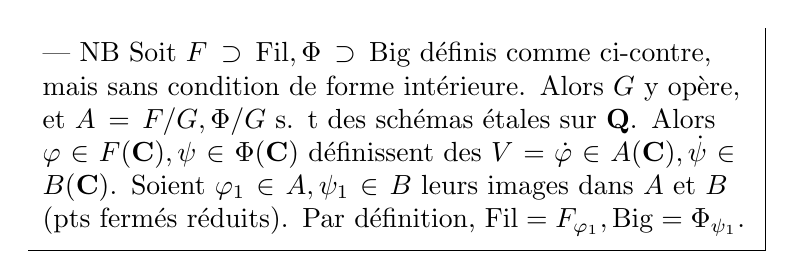
\begin{tikzpicture}
\node[align=left,text width=9cm,inner sep=5pt] (n) {--- NB Soit $F\supset\mathrm{Fil},\Phi\supset\mathrm{Big}$ définis comme ci-contre, mais sans condition de \unsure{forme intérieure}. Alors $G$ y opère, et $A=F/G,\Phi/G$ \unsure{s. t} des schémas \uline{\unsure{étales}} sur $\mathbf Q$. Alors $\varphi\in F(\mathbf C),\psi\in\Phi(\mathbf C)$ \deleted{définissent} des \unsure{$V=$} $\dot\varphi\in A(\mathbf C),\dot\psi\in B(\mathbf C)$. Soient $\varphi_1\in A,\psi_1\in B$ leurs images dans $A$ et $B$ (pts fermés réduits). Par définition, $\mathrm{Fil}=F_{\varphi_1},\mathrm{Big}=\Phi_{\psi_1}$.};
\draw (n.south west)--(n.south east)--(n.north east);
\end{tikzpicture}}}
\figure{\begin{tikzpicture}\draw[->] (0,0) .. controls (-.05,.3) and (-.2,.4) .. (-.55,.4);\end{tikzpicture}}

\margin{\uline{NB} Si on a $\varepsilon:\deleted{\unsure{G_m}}G'\longrightarrow G_m$ on a $(\varepsilon|B'/U')\circ j'=\mathrm{id}$. donc $j'$ mon. Si $H'\subset B'$ est l'image inverse de $\operatorname{Im}j'$ dans $B'$, alors \deleted{\unsure{le tout}} $j'$ est \inserted{donc} connu quand on connaît $H'$.}

\[
P\times P'\longrightarrow P'',\quad P'\times P''\longrightarrow P,\quad P''\times P\longrightarrow P',\qquad Q\subset P'
\]

\diagram{\begin{tikzcd}\mathrm{Big}\arrow[r,"p"] & \mathrm{Fil}\end{tikzcd}}
\deleted{\unsure{a}}
fibration, faisant de $B$ un torseur sur $\mathrm{Fil}$, de gr. $U_{\mathrm{Fil}}$, un groupe unipotent défini sur $F$, de dimension relative égale à $\dim U'$. $\mathrm{Fil}$ est de dim égale à $\dim G'/B'$, $\mathrm{Big}$ est de dim égale à $\dim G'/B'+\dim U'=\dim G'/L'$, \unsure{i.e.} $L'=\operatorname{Centr}(j'_0)$, $j'_0:G_{m_k}\longrightarrow H'$ relevant $j'$.

\margin{\figure{\begin{tikzpicture}
\node[draw,rounded corners=10pt,align=left,text width=8cm,inner sep=5pt] (a) {en fait, $\dot\varphi,\dot\psi$ sont dans $A(k),B(k)$ donc dans $A(k_1),B(k_1)$, où $k_1$ est la clôture alg. de $\mathbf Q$ dans $k$. D'ailleurs $F\longrightarrow\Phi$ induit $A\overset\sim\longrightarrow B$, donc};
\node[draw,align=left,text width=8cm,inner sep=5pt,anchor=north] at (a.south) {\unsure{autr. explicité en termes du groupe de Dynk. associé au réseau cor.} $\Gamma$ avec $W$ (Weyl) agissant : on \unsure{fera} $\Gamma/W$ par autom. extérieures....};
\end{tikzpicture}}}

On a un diagramme commutatif
\diagram{\begin{tikzcd}
P''\arrow[d,"\deleted{\unsure{q}}r"'] & P\arrow[d,"q"]\\
\mathrm{Big}_k\arrow[r,"p_k"'] & \mathrm{Fil}_k
\end{tikzcd}}
\[
\boxed{\begin{array}{l}\varphi=q(\alpha)\in\mathrm{Fil}(\mathbf C)\\\psi=r(\gamma)\in\mathrm{Big}(\mathbf C)\end{array}}
\qquad [\varphi=p(\psi)]
\]
\margin{$\dim G=g$\quad $\dim U'=u$\quad $\dim B'=b$\quad $\dim L'=\ell$\quad $(u+\ell=b)$}

\diagram{\begin{tikzcd}[row sep=small,column sep=small,execute at end picture={\draw ([xshift=-5pt,yshift=-5pt]current bounding box.south west) rectangle ([xshift=5pt,yshift=5pt]current bounding box.north east);}]
 & k(\alpha,\beta)=k(\beta,\gamma)=k(\gamma,\alpha)=K\arrow[dl,no head,"\leq u"']\arrow[dd,no head,"\leq u"]\arrow[ddr,no head,"\leq g"] & & \\
k(\gamma)\arrow[dd,no head,"\leq\ell"'] & & & \\
 & k(\alpha)\arrow[dd,no head,"\leq b"] & k(\beta)\arrow[ddd,no head,"\leq u"] & \\
k(\psi)\arrow[dr,no head,"\leq u" description]\arrow[dd,no head,"\mathrm{comp}"'] & & & \\
 & k(\varphi)\arrow[dr,no head,"\leq g-b" description]\arrow[dd,no head,"\mathrm{comp}"] & & \\
\mathbf Q(\psi)\arrow[dr,no head,"\leq u"'] & & k\arrow[dd,no head]\arrow[r,no head] & \substack{\mathbf Q(\varphi_1)\\\deleted{\unsure{\mathbf Q(\psi_1)}}=\mathbf Q(\varphi_1)}\\
 & \mathbf Q(\varphi)\arrow[dr,no head,"\leq g-b"] & & \\
 & \deleted{\unsure{\mathbf Q}} & \mathbf Q\arrow[uur,no head,"\mathrm{alg}"'] &
\end{tikzcd}}
\margin{\figure{\begin{tikzpicture}\node[draw,ellipse] {$\mathbf Q(\varphi_1)$ est \uline{indépendant}};\end{tikzpicture}} du plongement de $k$ dans $\mathbf C$, \unsure{donc} \illegible{3} \unsure{définit} \illegible{2} \unsure{du motif}.}
\[
\deleted{\unsure{K\subset k(\alpha)}}K\subset\deleted{\unsure{k(\alpha)}}\mathbf Q(k(\alpha),\overline{k(\alpha)})
\]
\[
(2i\pi)^n\in k(\alpha)\quad\text{si}\quad\mathbf Q(-n)\in\operatorname{Ob}\mathcal M
\]

\figure{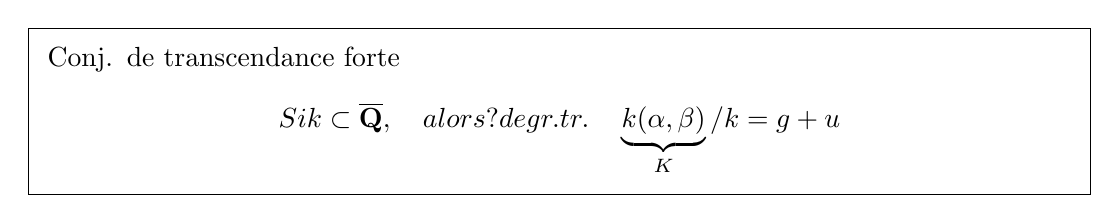
\begin{tikzpicture}
\node[draw,align=left,text width=13cm,inner sep=7pt] {
\uline{Conj. de transcendance forte}
\[
\text{Si } k\subset\overline{\mathbf Q},\quad\text{alors ? degr. tr.}\quad\underbrace{k(\alpha,\beta)}_K/k=g+u
\]
};
\end{tikzpicture}}
\[
\Longrightarrow\left\{\begin{array}{l}
\text{deg. tr.}\ k(\alpha)/k=g\\
\text{deg. tr.}\ k(\beta)/k=u\\
\text{deg tr.}\ k(\gamma)/k=g\\[.5em]
\text{deg. tr.}\ K/k(\beta)=g,\quad\text{et}\\
\text{deg tr.}\ K/k(\alpha)=\text{deg tr.}\ K/k(\gamma)=u\\[.5em]
\text{deg tr}\ \mathbf Q(\varphi)/\mathbf Q=g-b\\
\text{deg tr.}\ \mathbf Q(\psi)/\mathbf Q=g-b+u=g-\ell
\end{array}\right.
\]
\margin{10}
\scanpage{12}
\deleted{\unsure{fixe, mettons} $\mathbf C$ \unsure{ici}) sont déterminés à \unsure{cat.} alg. près. \unsure{N. m.} Nous \unsure{examinons} la

\uline{Conjecture}\inserted{\uline{transcendance}} Si $k$ est \unsure{quasi-modulaire|quasi-minimal} pour $M$, alors
\[
\operatorname{deg\,tr}(k(g_0))=\dim G^{\unsure{u}}\quad(=\dim G-1),
\]
i.e. $\unsure{\xi_0|g_0}$ \inserted{(localisé en $g_0$)} est un point \uline{maximal} de $G^{\unsure{u}}$ (du moins si $G$ donc $G^{\unsure{u}}$ connexe).}

\margin{\unsure{calcul} pour courbes elliptiques à invariant transcendant et $\tau$ algébrique.....}

\deleted{\uline{Corollaire.} \inserted{\figure{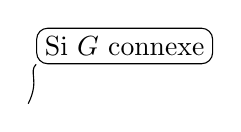
\begin{tikzpicture}[baseline=(n.base)]\node[draw,rounded corners=4pt,inner sep=3pt] (n) {Si $G$ connexe};\draw (n.south west) .. controls +(-.1,-.1) and +(.15,.3) .. ++(-.1,-.5);\end{tikzpicture}}} $G^{\unsure{u}}$ est le groupe algébrique engendré par $g_0$. Donc $G$ est le groupe algébrique engendré par $g_0$ et $j(G_m)$ (les homothéties). Enfin $G$ est engendré sur $k$ par $g$ si $G^{\unsure{u}}$ est $\frac12$ simple et $\pi$ \unsure{non|un} \unsure{algébrique} sur $k$ \deleted{\illegible{1}} ...}

\margin{et en général \deleted{\unsure{$G^u$}\quad\unsure{R un alg.}\quad\unsure{sur $k$ ?}}}

\deleted{Contient le th. de Schneider, pour les courbes elliptiques sans mult. complexe. En fait, il signifie que le degré de transc. du système
\[
\begin{array}{cccc}
(\unsure{\zeta|\xi}^{-1}\omega_1,&\unsure{\zeta|\xi}^{-1}\omega_2,&\unsure{\zeta|\xi}^{-1}\eta_1,&\unsure{\zeta|\xi}^{-1}\eta_2)\\
\text{''}&\text{''}&\text{''}&\text{''}\\
\omega'_1&\omega'_2&\eta'_1&\eta'_2
\end{array}
\]
sur $\mathbf Q$ est $3$ \deleted{\unsure{est}} (la seule relation étant $\omega'_1\eta'_2-\omega'_2\eta'_1=1$, \unsure{c.o.} l'équation de $G^{\unsure{u}}=\mathrm{SL}(2)\subset G=\mathrm{GL}(2)$) pour une courbe elliptique sans mult. complexe définie sur un corps de nbs alg. (disons sur $\overline{\mathbf Q}$).

Si l'invariant $j$ est transcendant, on \unsure{trouvera} que $(j,\omega'_1,\omega'_2,\eta'_1,\eta'_2)$ ont le degré de \uline{trans. $4$} sur $\mathbf Q$.}
\margin{11}
\scanpage{13}
\uline{Questions sur courbes elliptiques} sur $\overline{\mathbf Q}$.

Soit $C$ une telle courbe, $G$ son groupe de Galois motivique [$G\unsure{\simeq|\equiv}\mathrm{GL}(2,\mathbf Q)$ ou $G=\prod_{K/\mathbf Q}G_m$, $K$ le corps de multiplication complexe]. Soit $g\in G(\mathbf C)/G(\overline{\mathbf Q})$ définissant l'application du viseur transcendant de Betti dans celui de De Rham.

a) $\mathbf Q(g)$ de degré de transcendance égal à $\dim\unsure{G|C}$ ($4$ ou $2$)?

b) Soit $T$ le lieu de $g$ sur $G_{\overline{\mathbf Q}}$, \deleted{$\unsure{T=C}$} qu'on peut supposer (par translation à droite) contenir $e$, et soit $H$ le groupe engendré \deleted{et} par $T$. \deleted{et ses conjugués} A-t-on \deleted{\unsure{toujours}} $H=G$

c) Soit \deleted{$\unsure{g\in H_{\overline{\mathbf Q}}=G'_{\overline{\mathbf Q}}}$ \unsure{le conjugué par une courbe}} \inserted{$h\in\mathbf C/\overline{\mathbf Q}$ [quotient} additif) définissant le splitting transcendant (via H. de Hodge) de De Rham. Peut-on avoir $h\in\overline{\mathbf Q}$, ou $h$ est-il tjrs transcendant sur $\mathbf Q$ [\uline{cas où} $C$ \uline{n'a pas de multiplication complexe}]

\margin{\figure{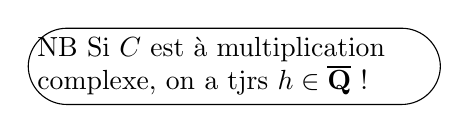
\begin{tikzpicture}\node[draw,rounded corners=14pt,text width=5cm,align=left] {\uline{NB} Si $C$ est à multiplication complexe, on a tjrs $h\in\overline{\mathbf Q}$ !};\end{tikzpicture}}}
\margin{12}
\scanpage{14}
Le foncteur de Hodge sur la catégorie des motifs.

(\uline{Comparaison des deux \unsure{fonct.|fonc.} alg. et transcendants}).
\margin{13}
\scanpage{15}
\uline{Comparaison de classes fondamentales}\quad analytiques ($=$ alg) et topologiques ($=$ transc.).

$X$ variété \deleted{\unsure{analyti}} holomorphe

$Y$ ss-variété holomorphe de codim $p$ partout.

$\underline\Omega_X^\bullet$ résolution de $\mathbf C$

\diagram{\begin{tikzcd}[row sep=large,column sep=small]
\underline H_Y^{2p}(X,\mathbf Z)\arrow[r,"i", "\text{can}" description] & \underline H_Y^{2p}(X,\mathbf Z)\otimes_{\mathbf Z}\mathbf C\arrow[r,"\sim", "\text{can}" description] & \underline H_Y^{2p}(X,\mathbf C)\arrow[r,"\sim", "\text{De Rham (i.e. can)}" description] & \underline{\underline H}_Y^{2p}(X,\underline\Omega_X^\bullet) & \\
 & & & & \underline H_Y^p(X,\underline\Omega_X^p)\arrow[ul,"\text{suite spectrale}"]\\
\mathbf Z_{\unsure{Y|\deleted{X}}}\arrow[uu,"p_{\mathrm{top}}^{\mathbf Z}"',"\sim"]\arrow[r,hook] & \mathbf C_Y\arrow[r,equal]\arrow[uu,phantom,"\deleted{\unsure{p^{\mathbf C}}}" description] & \mathbf C_Y\arrow[uu,"p_{\mathrm{top}}^{\mathbf C}"',"\sim"]\arrow[r,"\frac1{(2i\pi)^p}"'] & \mathbf C_Y\arrow[uu,"p_{\mathrm{an}}^{\mathbf C}"',"\sim"]\arrow[ur,"\uuline{\text{résidu}}"'] & \\
 & & \deleted{\unsure{\underline H_Y^p(X,\underline\Omega_X^p)}}\deleted{\arrow[uuu,"\unsure{\rotatebox{90}{$\sim$}}" description]\arrow[ur]} & &
\end{tikzcd}}
\margin{$p_{\mathrm{top}}^{\mathbf Z}:$ Poincaré topologique local}

\margin{\figure{\begin{tikzpicture}
\node[text width=5.8cm,align=left,inner sep=6pt] (n) {\uline{Poincaré analytique local} [défini par voie ess. alg.]\par\unsure{si|à} $f_1\ldots f_p$ est un syst. d'équations locales de $Y$, on prend la section $\dfrac{df_1}{f_1}\wedge\cdots\wedge\dfrac{df_p}{f_p}$ de $\underline H_Y^p(\underline\Omega_X^p)$)};
\draw[->] ($(n.north)+(-.5,.9)$) .. controls +(1,0) and +(.3,.5) .. (n.north);
\draw ($(n.north west)+(-1,0)$) .. controls +(.8,.2) and +(0,.4) .. ($(n.west)+(-.15,0)$) -- ($(n.south west)+(-.15,0)$) -- (n.south east);
\end{tikzpicture}}}

On est ramené au cas où $Y$ est réduit à un pt $a$ (prendre une \deleted{section} $X'^{n-p}$ transverse à $Y$ en un pt) et par cup-produit au cas où $X$ est de dim $1$, \unsure{disons} un disque de centre \unsure{$x$|$a$}.

[NB. à priori, \unsure{c'est acquis par ce qui précède} qu'il \unsure{le}\inserted{existe un} multiplicateur de la forme $\lambda^p$, $\lambda\in\mathbf C^*$ étant indépt de $X,Y,p$]. Alors on a

\diagram{\begin{tikzcd}[row sep=large,column sep=large]
H^1(X-a,\mathbf Z)\arrow[r]\arrow[d,phantom,"\rotatebox{90}{$\simeq$}" description] & H^1(X-a,\mathbf C)\arrow[r,"\sim"]\arrow[d,phantom,"\rotatebox{90}{$\simeq$}" description] & \underline{\underline H}^{1}(X-a,\underline\Omega_X^\bullet)\arrow[d,phantom,"\rotatebox{90}{$\simeq$}" description] & \\
H_a^2(X,\mathbf Z)\arrow[r] & H_a^2(X,\mathbf C)\arrow[r,"\sim"] & \underline{\underline H}_a^2(X,\underline\Omega_X^\bullet) & \\
\mathbf Z\arrow[u,"p_t^{\mathbf Z}"',"\sim"]\arrow[r] & \mathbf C\arrow[u,"p_t^{\mathbf C}"']\arrow[r,"\lambda"] & \mathbf C\arrow[u,"p_{\mathrm{an}}^{\mathbf C}"']\arrow[r] & H_a^1(X,\Omega_X^1)\arrow[ul,"\sim"]\quad\frac{dz}{z}
\end{tikzcd}}
\figure{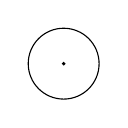
\begin{tikzpicture}\draw (0,0) circle (.45);\fill (0,0) circle (.025);\end{tikzpicture}}
\margin{14}
\scanpage{16}
\begin{center}A - 21 -\hfill n$^{\mathrm o}$ 413\end{center}

de $V$ dans $N$ comme étant un élément de $\operatorname{Hom}(U(\underline V);N)$ et noter $\widehat P(\underline V;N)$ le module ainsi défini, $\widehat P_+(\underline V;N)$ désignant le sous-module des applications linéaires nulles sur $U_0(\underline V)$. Ceci ne peut être gênant puisque dans le cas d'un module libre, il y a un isomorphisme canonique de l'un sur l'autre des deux modules notés $\widehat P_+(\underline V;N)$. Si $N=K$, on identifiera $\widehat P(\underline V;K)$ et $\widehat P(\underline V)$.

Soient $\underline V$ et $\underline W$ deux noyaux formels. Nous allons caractériser les applications linéaires de $U(\underline V)$ dans $U(\underline W)$ qui proviennent d'applications formelles de $\underline V$ dans $\underline W$ :

PROPOSITION 8.- \uline{Pour qu'une application linéaire} $\psi$ \uline{de} $U(\underline V)$ \uline{dans} $U(\underline W)$ \uline{soit de la forme} $\varphi_*$ \uline{avec} $\varphi\in\widehat P_+(\underline V;\underline W)$, \uline{il faut et il suffit que} $\psi(U_0(\underline V))=U_0(\underline W)$ \uline{et que} $\psi$ \uline{soit compatible avec les applications diagonales} \uline{(c'est-à-dire que}
\[
(\psi\otimes\psi)\circ\mathrm T=\mathrm T\circ\psi).
\]

Que les conditions soient nécessaires résulte de la prop. 6. La prop. 7 montre d'ailleurs que si $\varphi$ existe, elle est unique. Pour démontrer l'existence de $\varphi$, on se ramène en prenant des cartes formelles, au cas de noyaux formels définis par des modules libres $M$ et $N$. Soit alors $(e_i)_{i\in I}$ une base de $M$, $(e'_j)_{j\in J}$ une base de $M'$, et posons :
\[
(30)\qquad \psi(e_\alpha)=\sum a_{\alpha,\beta}\,e'_\beta
\qquad (a_{\alpha,\beta}\in K).
\]
\margin{\figure{
\begin{tikzpicture}[scale=.5]\draw[line width=1.7pt] (0,.9)--(.3,.5);\draw[line width=1pt] (-.16,.05)--(-.16,-.04);\draw[line width=1.4pt] (0,.03)--(0,-.12);\end{tikzpicture}}}
La condition $\psi(U_0(\underline V))=U_0(\underline W)$ entraîne
\[
(31)\qquad a_{0,\beta}=0\quad\text{pour }|\beta|\geq 1\,,\quad a_{0,0}\neq 0.
\]
La compatibilité de $\psi$ avec les applications diagonales donne :
\[
(32)\qquad a_{\alpha,\beta_1+\beta_2}=\sum_{\alpha_1+\alpha_2=\alpha}a_{\alpha_1,\beta_1}\,a_{\alpha_2,\beta_2}.
\]
\margin{15}
\scanpage{17}
\margin{\unsure{faire le raisonnement}}
\margin{\figure{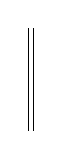
\begin{tikzpicture}\draw (0,0)--(0,1.3);\draw (.07,0)--(.07,1.3);\end{tikzpicture}}}
Alors on voit que $P_{\mathrm{an}}(1_Y)$ est la classe de \unsure{Coh.} sur $X-a$ représenté par la forme diff. $\dfrac{dz}{z}$, et par suite \deleted{\unsure{on a}} si $P_{\mathrm{an}}(1_Y)=\lambda P_{\mathrm{top}}(1_Y)$, on a
\diagram{\begin{tikzcd}[column sep=small,row sep=small]
\lambda={} & \displaystyle\int_C P_{\mathrm{an}}\unsure{(}1_Y) & {}={} & \displaystyle\int_C\frac{dz}{z} & {}=2i\pi \\
& & \begin{gathered}\text{cercle unité }\deleted{\text{\unsure{coord.}}}\\\text{orienté.}\end{gathered}\arrow[ul,bend left=15]\arrow[ur,bend right=15] & &
\end{tikzcd}}
Donc
\[
\boxed{P_{\mathrm{an}}\left(\frac{1}{2i\pi}1_Y\right)=P_{\mathrm{top}}(1_Y)}
\]
\[
\boxed{\left\{\begin{aligned}
P_{\mathrm{top}}(1_Y)&=\frac{1}{2i\pi}P_{\mathrm{an}}(1_Y)\\
P_{\mathrm{an}}(1_Y)&=2i\pi P_{\mathrm{top}}(1_Y)
\end{aligned}\right.}
\]
\figure{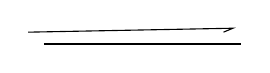
\begin{tikzpicture}\draw (0,0)--(2.6,.05)--(2.48,0);\draw (.2,-.15)--(2.7,-.15);\end{tikzpicture}}

\deleted{\uline{\unsure{Gén.}}} Considérons le diagramme.
\diagram{\begin{tikzcd}[column sep=large,row sep=large]
H^{i+p}_{\unsure{\alpha|Z}}(X,\mathbf Z)\arrow[r,leftrightarrow] &
H^{\deleted{\unsure{*}}\inserted{i}+p}_{\unsure{Z}}(X,\mathbf C)\arrow[r,no head,"\sim","\text{De Rham}" description] &
H^{\deleted{\unsure{*}}\inserted{i}+p}(X,\Omega_X^\bullet)\\
H^{\deleted{\unsure{*}}\inserted{i}}_{\unsure{Z}}(Y,\mathbf Z)\arrow[r]\arrow[u,"P_{\mathrm{top}}"'] &
H^{\deleted{\unsure{*}}\inserted{i}}_{\unsure{Z}}(\deleted{\unsure{X}}\inserted{Y},\mathbf C)\arrow[u,"P_{\mathrm{top}}"']\arrow[r,no head,"\substack{\deleted{\text{\unsure{can.}}}\\\sim}","\frac{1}{(2i\pi)^p}\text{can.}"'] &
\underline{\underline H}^{\deleted{\unsure{*}}\inserted{i}}_{\unsure{Z}}(\deleted{\unsure{X}}\inserted{Y},\Omega^\bullet_{\deleted{\unsure{X}}\inserted{Y}})\arrow[u,"P_{\mathrm{an}}"']
\end{tikzcd}}
\uline{Il est commutatif}, i.e. la formule ci-dessus est valable \uline{globalement}, et en remplaçant $1_Y$ par une classe de Coh. quelc. \unsure{Par raison de la comm. de}
\margin{16}
